\documentclass{./assets/wfis}
\usepackage[utf8]{inputenc}
\usepackage{amsmath}
\usepackage{tabularx}
\usepackage[hidelinks]{hyperref}
\usepackage{afterpage}
\usepackage[sorting=none]{biblatex} 
\addbibresource{assets/references.bib}

\usepackage{framed}
\usepackage{listings}
\usepackage[most]{tcolorbox}
\usepackage{hyphenat}
\usepackage{amsmath}

\usepackage{graphicx}
\usepackage{subcaption}
\usepackage{url}
\usepackage{breakurl}
\def\UrlBreaks{\do\/\do-}

% BEGIN CODE
\usepackage{algorithm}
\usepackage{algpseudocode}
\usepackage{listings}
\usepackage{color}
\usepackage{xcolor}

\definecolor{dkgreen}{rgb}{0,0.6,0}
\definecolor{gray}{rgb}{0.5,0.5,0.5}
\definecolor{mauve}{rgb}{0.58,0,0.82}

\lstset{
    frame=tb,
  language=Python
  captionpos=b,                    % sets the caption-position to bottom,
  % aboveskip=3mm,
  % belowskip=3mm,
  showstringspaces=false,
  columns=flexible,
  basicstyle={\small\ttfamily},  
  % numbers=none,
  numbers=left,
  numberstyle=\tiny\color{gray},
  keywordstyle=\bfseries,
  commentstyle=\color{gray},
  stringstyle=\color{mauve},
  breaklines=true,
  breakatwhitespace=true,
  tabsize=3
}
% END CODE

\newtcolorbox{boxA}{
    fontupper = \bf,
    boxrule = 1.5pt,
    colframe = black % frame color
}

\begin{document}

\tytul{Wykrywanie zmian stanu skupienia przy użyciu aparatu EEG}
\autor{Mateusz Kojro}
\nralbumu{389105}
\promotor{dr hab. Krzysztofa Wardy}
\katedra{Teorii Ciała Stałego}
\kierunek{informatyka}
\specjalnosc{informatyka stosowana}
\typpracy{inżynierska}
\specjalizacja{Algorytmy i Programowanie}

\stronatytulowa

\begin{abstract}
Praca prezentuje proces opracowania oraz ewaluacji modelu pozwalającego na wykrywanie stopnia skupienia człowieka za pomocą elektroencefalografii (EEG). W tym celu przygotowano dedykowane oprogramowanie pozwalające na nagrywanie sygnału EEG podczas wykonywania prezentowanych zadań matematycznych. Następnie przeprowadzono kampanię badawczą na próbce ochotników, analizując zebrane dane oraz testując wydajność lasów losowych, oraz głębokich, konwolucyjnych i rekurencyjnych sieci neuronowych.
\end{abstract}

\chapter{Wstęp}
Ludzki układ nerwowy składa się z miliardów komórek nerwowych, połączonych w gęstą siatkę pokrywającą całą powierzchnię ludzkiego ciała tworząc niezwykle skomplikowany system odpowiadający za różnorodne aspekty naszego życia: od tak prostych jak poruszanie pojedynczymi mięśniami, przez dekodowanie rzeczywistości z nieskończonego strumienia impulsów dochodzących z wszystkich zmysłów, aż po kontrolowanie uczuć tak skomplikowanych jak ciekawość. Na czele tego niezwykłego wynalazku ewolucji stoi mózg, zagadka, której naukowcy i filozofowie poświęcali swoje życia od czasów sławnego eksperymentu myślowego Decartesa. Dopiero niedawno, opierając się na pracy wielu osób w niezliczonych dziedzinach współczesnej nauki, możliwe stało się rozwikłanie części tej niesamowitej tajemnicy. Kontynuując tę ścieżkę, poniższa praca przedstawia opracowanie oraz ewaluacje modelu klasyfikującego stan skupienia, za pomocą badania reakcji na bodziec z użyciem elektroencefalografii. 

W ramach projektu przygotowano układ eksperymentalny (sekcja \ref{aparatura-pomiarowa}), przeprowadzono kampanię badawczą na próbce 19 osób (sekcja \ref{procedura-badan}), której wyniki zostały następnie poddane analizie tradycyjnymi metodami statystycznymi (sekcja \ref{analiza-klasyczna}), uwzględniając zmienne zakłócające (sekcja \ref{zmiennne-zaklucajace}) oraz algorytmami uczenia maszynowego (sekcja \ref{uczenie-maszynowe}). Dyskusję wyników zaprezentowano w sekcji \ref{dyskusja}.

\section{Motywacja}
Uczenie maszynowe pozwala rozwiązywać problemy, w których relacja pomiędzy wejściami i wyjściami algorytmu jest zbyt skomplikowana, aby w praktyczny sposób przedstawić ją jako serie warunków. Nie dziwnym jest więc, że znajdują one coraz większe zastosowanie w dziedzinach medycyny, biologii i chemii, pozwalając na tak niesamowite osiągnięcia jak np. diagnozowanie raka płuc \cite{li_machine_2022} czy zwijanie białek (ang. \textit{protein folding}) \cite{jumper_highly_2021}. Jednocześnie mimo wczesnych sukcesów \cite{some comparasion}, próby diagnozy chorób psychologicznych za pomocą badań obrazowych są na stosunkowo niskim poziomie rozwoju \cite{badania adhd i podobne}. Jako krok w drodze do opracowania tego typu metod, niniejsza praca zawiera porównanie skuteczności wybranych metod badawczych na prostszym problemie oceny uwagi człowieka. Decyzja o wykorzystaniu elektroencefalografii podyktowana została łatwym dostępem do aparatury pomiarowej, możliwością stosunkowo prostego zbierania znaczących ilości danych oraz brakiem konieczności wykonywania badań w środowisku laboratoryjnym.

\section{Przegląd literatury}
Możliwość wykorzystania badania EEG w celu analizy stanu mentalnego pacjenta zaprezentowana została między innymi przez Kaushika i in. \cite{kaushik_decoding_2022}. Dodatkowo Guo i in. \cite{guo_detection_2018} pokazali, że możliwe jest klasyfikowanie stanu skupienia kierowcy w symulowanych warunkach. Wysoką skuteczność algorytmów uczenia maszynowego takich jak maszyny wektorów nośnych czy uczenie głębokie do analizy wyników elektroencefalografii udowodnili de Taillez i in. \cite{de_taillez_machine_2020}. Rozpoczęto również prace nad zastosowaniem algorytmów uczenia maszynowego w celu diagnozy innych jednostek chorobowych takich jak ADHD, dysleksja czy schizofrenia \cite{ahire_comprehensive_2022, joshi_review_2021, clarke_eeg_2002}.

\chapter{Podstawy teoretyczne}
% \section{Model działania mózgu}
% Pierwsze modele pracy mozgu stworzone zostaly juz w ... jednak dopiero

Informacje w mózgu przekazywane i przetwarzane są za pomocą tzw. potencjałów czynnościowych – chwilowych impulsów, podczas których napięcie wewnątrz komórki stanowczo wzrasta (xxxx). Impuls taki zostaje wygenerowany, gdy czasowo skalowana suma napieć na ,,wejściach'' komórki (dendrytach) przekroczy pewien poziom (xxxx). W takiej sytuacji generowane jest napięcie, które następnie przekazywane jest za pomocą aksonu do kolejnych komórek (xxxxx). W dużym uproszczeniu potencjał komórki można więc zapisać równaniem \ref{eq:napiecie-komorki}, gdzie $d_i(t)$ to napięcie na dendrycie $i$ w czasie $t$.
\begin{equation}\label{eq:napiecie-komorki}
    \text{Potencjał komórki} \approx 
    \begin{cases} 
      70mV & \sum_i d_i(t) > \text{Napięcie progowe}  \\
      -30mV &  \text{inaczej}
   \end{cases}
\end{equation}

% - wspomniec huxley model
% - bilions of those interactions form a working brain
% - i want the plot of the cell potential

\section{Metody badania aktywności mózgu}
W 1884 włoski psycholog Angelo Mosso wygłosił wykład \cite{sandrone_weighing_2014} w którym przedstawił swój nowy wynalazek, stół pozwalający na balansowanie dorosłego mężczyzny na pojedynczym punkcie podparcia w celu obserwacji przepływu krwi w ludzkim ciele. 

Pacjent, leżąc na plecach w stanie równowagi, poddawany zostawał dzianiu bodźca mającego na celu pobudzenie działania mózgu (z początku był to dźwięk, później tekst gazety czy podręcznika do matematyki \cite{sandrone_weighing_2014}), co miało spowodować napływ większej ilości krwi do mózgu, a przez to pochylenie urządzenia w stronę głowy badanego. Była to pierwsza udokumentowana próba naukowego mierzenia aktywności mózgu\footnote{Wyniki jego badan zostały poddane poważnej wątpliwości w pracy opublikowanej przez M. F. Lowe \cite{lowe_application_1936} w 1936 roku – według niego wykrywane zmiany fizjologiczne nie mogą być jednoznacznie powiązane z aktywnością mózgu}.

Mimo końcowego niepowodzenia, fascynująca jest ilość podobieństw pomiędzy eksperymentami przeprowadzonymi przez Mosso, a badaniami prowadzonymi przez współczesnych naukowców. Od metodologii badania aktywności mózgu, opierającej się na tym samym fenomenie zwiększonego ciśnienia krwi co PET (ang. \textit{positron emission tomography}) czy fMRI (ang. \textit{functional magnetic resonance imaging}), po uwagę zwróconą na eliminowanie zmiennych zakłócających takich jak bicie serca podczas elektroencefalografii czy wdechy i wydechy podczas badania Mossa.

Aktualnie stosowane metody pomiaru aktywności mózgu, podzielić można ze względu na wykorzystywany fenomen – badanie przebiegu krwi lub pól elektromagnetycznych generowanych przez oddziaływania neuronów. Do pierwszej kategorii należą badania takie jak PET (przepływ krwi mierzony jest za pomocą obserwowania promieniowania wydzielanego przez radioaktywny izotop podany dożylnie) i fMRI wykorzystujące różnice we właściwościach magnetycznych hemoglobiny związane z jej utlenieniem. Największą zaletą tych metod jest wysoka dokładność przestrzenna, pozwalająca na tworzenie trójwymiarowych obrazów mózgu z dokładnością poniżej $1mm$. Po drugiej stronie  spektrum znajdują się natomiast badania wykorzystujące zjawiska elektromagnetyczne występujące w mózgu. Najpopularniejsze z nich to magnetoencefalografia (MEG) – badająca zmiany w polu magnetycznym i elektroencefalografia (EEG) – badanie zmian napięcia. 

\begin{figure}[h]
    \centering
    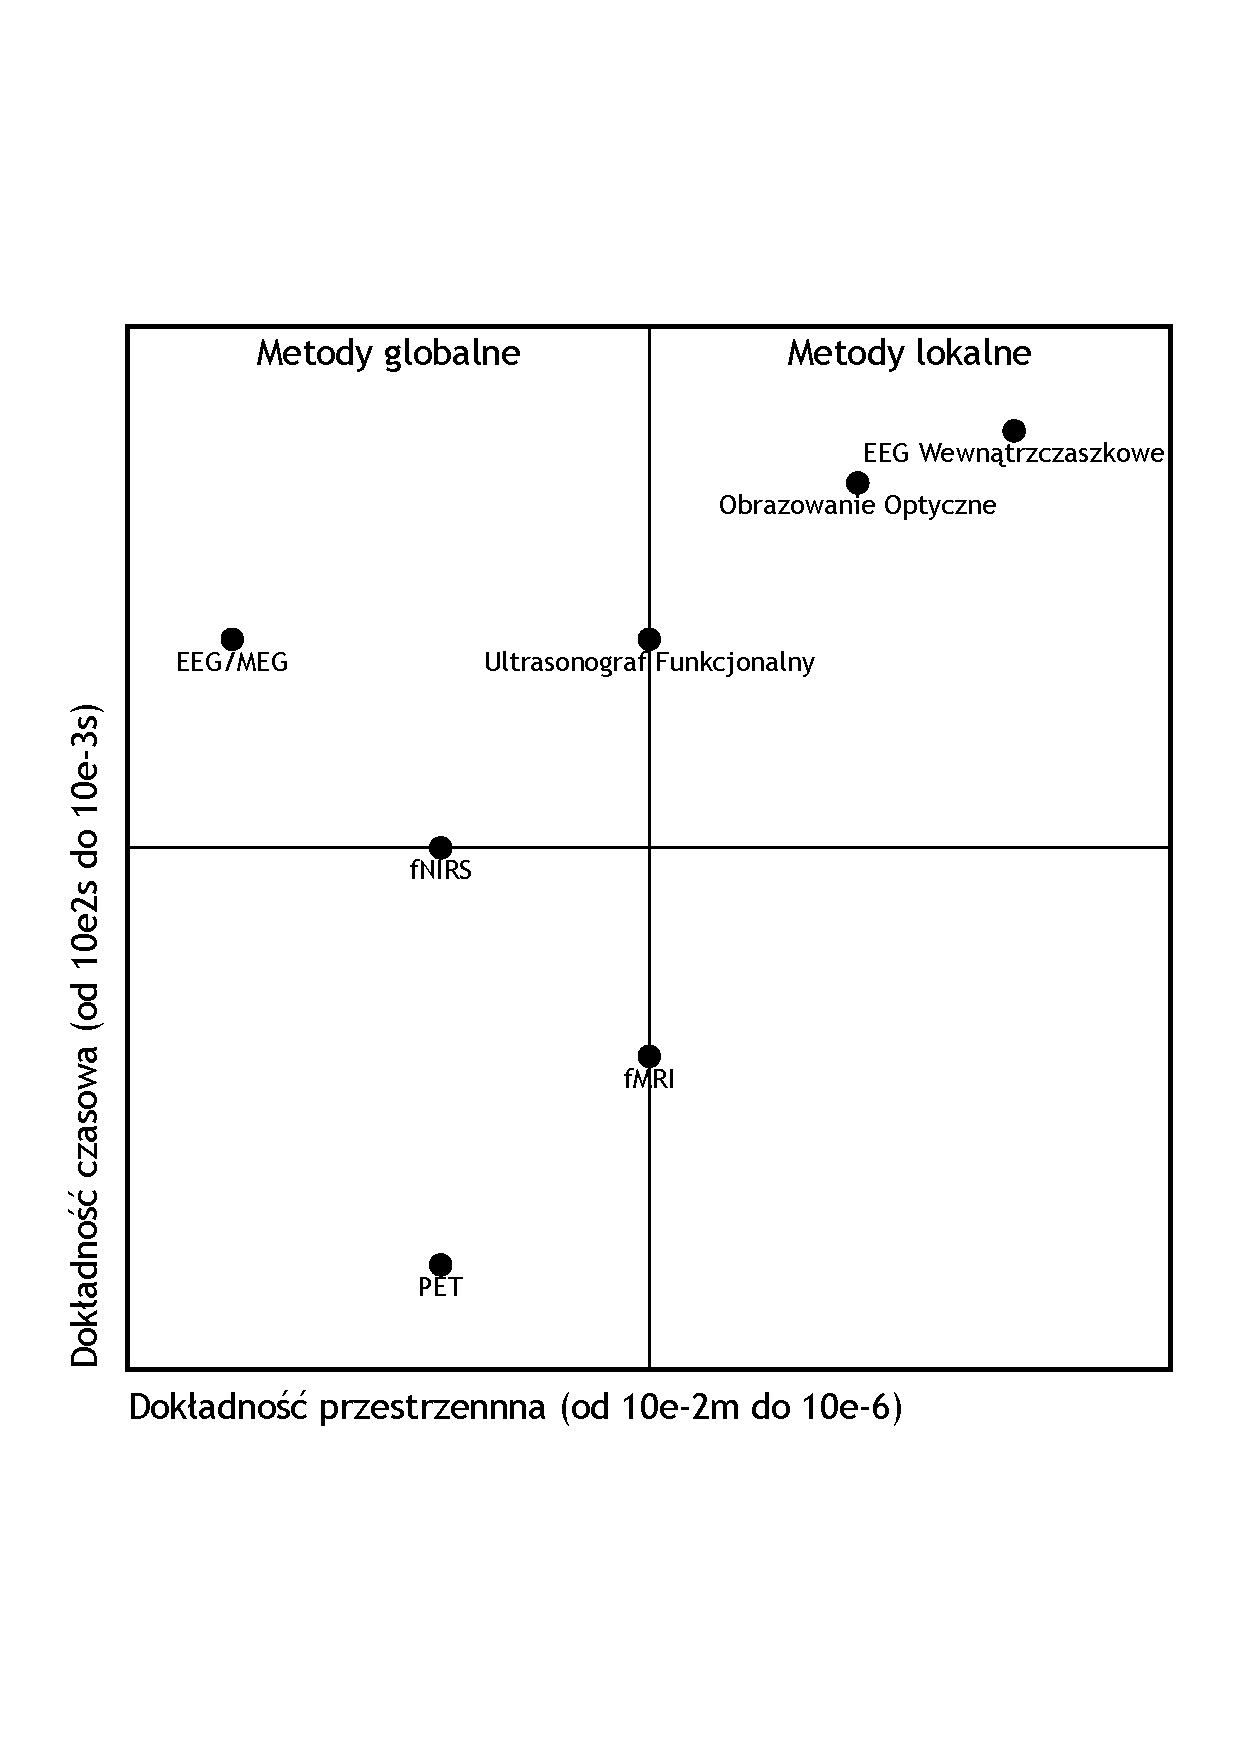
\includegraphics[width=0.75\columnwidth, trim={0 6cm 0 6cm}]{diagrams/brain_imaging.pdf}
    \caption{Porównanie metod badania mózgu ze względu na dokładność czasową i przestrzenną}
    \label{fig:brain-imaging-comparasion}
\end{figure}

\section{Elektroencefalografia}
Elektroencefalografia to badanie polegające na pomiarze potencjałów elektrycznych w różnych punktach na powierzchni czaszki pacjenta. Zebrane w ten sposób informacje pozwalają na określenie względnej aktywności różnych obszarów mózgu. Tradycyjnie wykorzystywana jest do diagnozowania schorzeń neurologicznych takich jak epilepsja, nowotwory mózgu czy zaburzenia snu.

\subsection{Mechanizm działania}
Układ nerwowy człowieka przekazuje oraz przetwarza informacje za pomocą impulsów elektrycznych (potencjałów czynnościowych) wytwarzanych w komórkach nerwowych (neuronach), z pomocą tzw. pompy sodowo-potasowej. Ze względu na dużą liczbę neuronów w ludzkim mózgu ($\approx10^9$\cite{herculano-houzel_human_2009}), ich niewielkie rozmiary, małe napięcie impulsu potencjału czynnościowego ($\approx100mV$\cite{biga_anatomy_2019}) oraz krótki czas jego trwania ($\approx2ms$\cite{biga_anatomy_2019}) niemożliwe jest badanie pracy pojedynczych neuronów, a jedynie średnich wartości milionów zsynchronizowanych impulsów na przestrzeni centymetrów. Ograniczenia te powodują, że różne obszary mózgu mogą być badane z różną dokładnością (najlepszą sprawność otrzymuje się w rejonach mózgu znajdujących się blisko powierzchni skóry zawierających dużą liczbę tzw. neuronów piramidowych – np. kora przedczołowa).

\subsection{Metodyka badania}
W zależności od specyfiki badania ważny jest dobór następujących parametrów bdadania 

\subsubsection{Rozmieszczenie oraz liczba elektrod}
Najbardziej popularnymi standardami pozycjonowania elektrod są tzw. międzynarodowe systemy $10$–$10$ i $10$–$20$\footnote{Wartości liczbowe w nazwie wywodzą się  z procentowego podziału czaszki – elektroda znajduje się co $10\%$ obwodu czaszki na osi przód – tył i co $20\%$ na osi prawo – lewo} \cite{herbert_h_jasper_report_1958} (przedstawiony na rysunku \ref{fig:10-20-system}). Stosowanie tych metod pozwala na stosunkowo łatwe powielanie i porównywanie wyników badań przeprowadzonych w różnych placówkach. Układy te najczęściej stosowane są w środowisku medycznym. 

\begin{figure}[h]
    \centering
    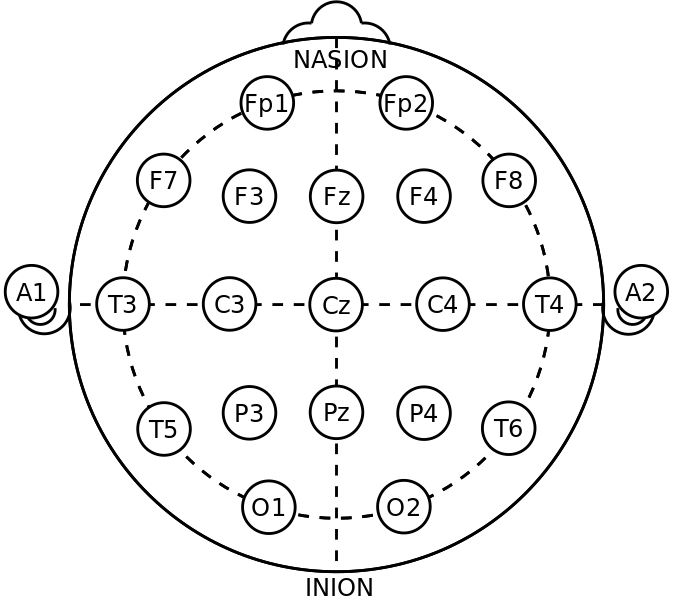
\includegraphics[width=0.5\columnwidth]{thesis/assets/10-20_system_electrodes.png}
    \caption[Rozmieszczenie elektrod w międzynarodowym systemie $10$-$20$]{Rozmieszczenie elektrod w międzynarodowym systemie $10$-$20$\footnotemark}
    \label{fig:10-20-system}
\end{figure}
\footnotetext{\href{https://commons.wikimedia.org/wiki/File:21_electrodes_of_International_10-20_system_for_EEG.svg}{
\begin{CJK}{UTF8}{}
\begin{Japanese}
トマトン
\end{Japanese}  
\end{CJK}124, Public domain, via Wikimedia Commons}}

Alternatywne metody rozmieszczenia elektrod stosowane są czasami w produktach komercjalnych z kategorii BCI (ang. \textit{brain computer interface}). Narzędzia te często ignorują standardy pozycjonowania elektrod i skupiają je na korze przedczołowej w celu optymalizacji stosunku kosztów do jakości zebranych danych. Przykładem urządzenia stosującego ten zabieg jest wykorzystany na potrzeby pracy zestaw Emotiv EPOC X \cite{emotiv_inc_epoc_nodate}. 


\subsubsection{Rodzaj elektrod}
Ze względu na jakość wyników, czas trwania badania oraz okoliczności towarzyszące badaniu konieczny jest dobór odpowiedniego typu elektrod. Najpopularniejsze z nich to:

\begin{itemize}
    \item \textbf{Elektrody żelowe} - zapewniają wysoki poziom komfortu oraz dokładności pomiarów; wymagają aplikacji specjalnego żelu przewodzącego, utrudniając prowadzenie badań.
    \item \textbf{Elektrody gąbkowe} - pozwalają na kompromis pomiędzy jakością zebranych danych, a łatwością aplikacji (żel przewodzący zamieniany jest na roztwór soli).
    \item \textbf{Elektrody suche} - oferują najniższy poziom komfortu oraz dokładności, w zamian za bardzo wysoką łatwość użycia.
\end{itemize}

\subsubsection{Montaż}
Podczas badania EEG montażem nazywa się konfigurację punktów odniesienia dla poszczególnych elektrod. Najbardziej popularnymi metodami są:
\begin{itemize}
    \item \textbf{Montaż sekwencyjny} – kanał danych jest definiowany przez różnicę potencjałów pomiędzy dwoma sąsiednimi elektrodami.
    \item \textbf{Montaż referencyjny} – wartość każdego kanału jest równa różnicy napięć pomiędzy daną elektrodą i elektrodą referencyjną.
    \item \textbf{Montaż średnio-referencyjny} – każdy kanał to różnica pomiędzy wartością danej elektrody i średniej wartości pozostałych elektrod. 
    \item \textbf{Montaż Laplace’a} – kanał danych jest definiowany jako różnica między wartością kanału i średniej ważonej sąsiednich elektrod.
\end{itemize}


\subsubsection{Badane częstotliwości}

W medycynie, ze względu na wysoki poziom złożoności, bezpośrednią analizę przebiegów czasowych potencjałów stosuje się niezwykle rzadko – standardową metodą jest porównywanie aktywności mózgu na określonych przedziałach częstotliwości (\autoref{tab:freqs}), tak na przykład aktywność w zakresie $\alpha$ wzrasta po zamknięciu oczu, a przedziale $\beta$ w trakcie ruchu \cite{britton_electroencephalography_2016}. 

\begin{table}[h]
    \centering
    \begin{tabular}{|c|c|c|}
        \hline
        Oznaczenie & Zakres częstotliwości \\
        \hline
        $\delta$ & $1$-$3$ Hz  \\
        $\theta$ & $4$-$7$ Hz \\
        $\alpha$ & $8$-$12$ Hz \\
        $\beta$  & $13$-$25$ Hz \\
        $\gamma$ & $>25$ Hz \\
        \hline
    \end{tabular}
    \caption{Typowe oznaczenia częstotliwości podczas badania EEG}
    \label{tab:freqs}
\end{table}

\chapter{Metody}

\section{Aparatura pomiarowa}\label{aparatura-pomiarowa}
% - w projekekcie napisalem ze to bedzie sterownik so i should make that clear
W celu przeprowadzenia badań opracowano aplikację webową pozwalającą na wyświetlanie bodźców na ekranie komputera (np. zadań matematycznych) oraz oprogramowanie serwerowe odpowiedzialne za sterowanie urządzeniem pomiarowym (Emotiv EPOCX lub innymi urządzeniami firmy Emotiv), zbieranie informacji na temat odpowiedzi użytkownika, oraz korelowanie ich w czasie z mierzonym sygnałem EEG.

\subsection{Oprogramowanie}
% - this should probably be pretty precise zeby nie bylo pytan czy to napewno jest praca inżynierska
% - info o tym gdzie i jak zapisujemy wyniki
% - info o konifguracji
Aplikacja stworzona na potrzeby badania składa się z dwóch komponentów. Formularza zbierającego informacje na temat uczestnika i okoliczności, w jakich był on badany (\autoref{formularz-dla-osoby-badanej}) oraz modułu pozwalającego na wyświetlanie pytań w określonym interwale, oraz oznaczenia momentu udzielenia odpowiedzi. Na rysunku \ref{fig:app-flow} przedstawiono diagram typowego procesu działania aplikacji.
\begin{figure}[h!]
    \centering
    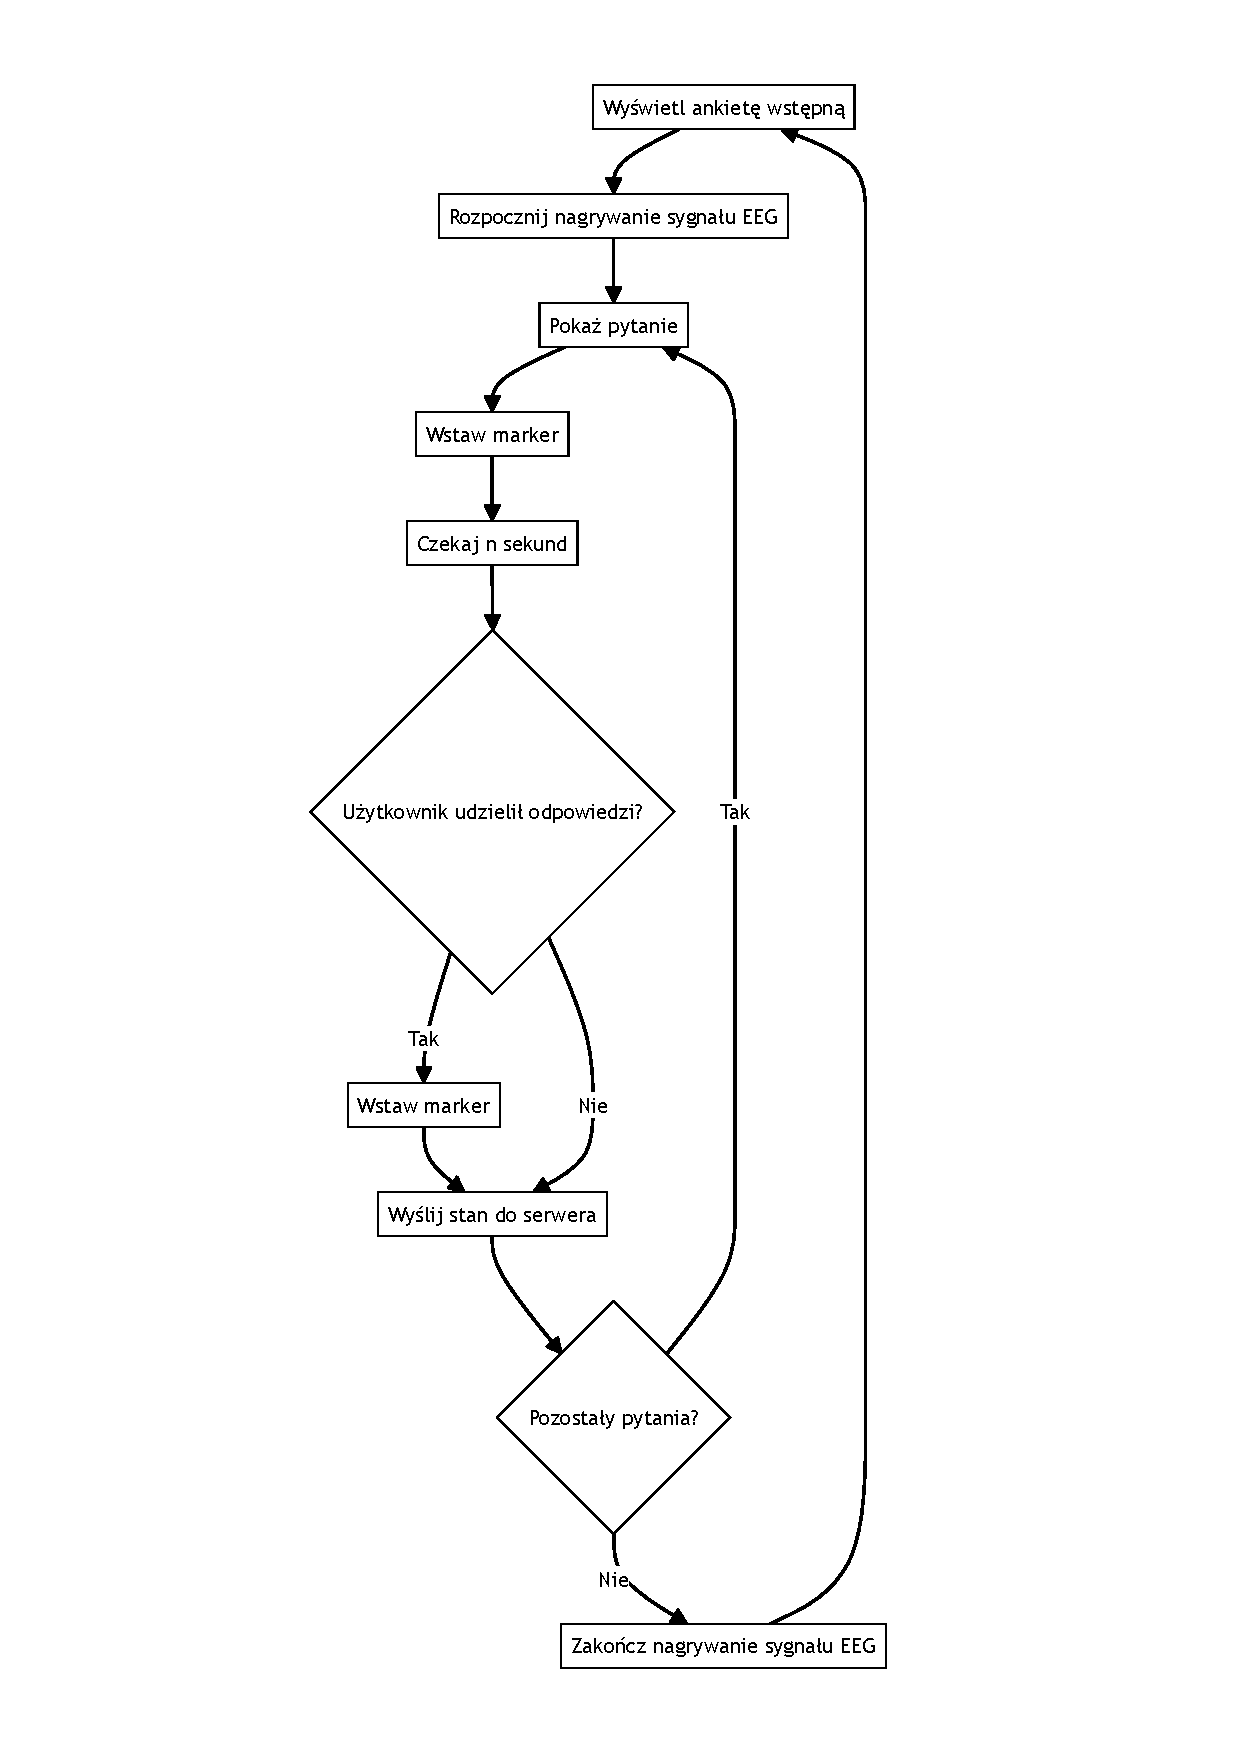
\includegraphics[width=\columnwidth]{diagrams/app_flow.pdf}
    \caption{Typowy proces działania aplikacji}
    \label{fig:app-flow}
\end{figure}
Całość oprogramowania serwerowego napisano w języku programowania \textit{Python} \cite{python_developers_python_2024} w wersji 3.9, używając biblioteki \textit{Flask} \cite{flask_developers_flask_nodate} do implementacji REST API. Komunikacja z urządzeniem pomiarowym odbywa się za pomocą protokołu WebSocket z wykorzystaniem pakietu \textit{websocket-client} \cite{liris_websocket-client_nodate}. Interfejs graficzny przygotowano z użyciem biblioteki \textit{htmx} \cite{htmx_developers_htmx_nodate}, a do renderowania działań matematycznych wykorzystano bibliotekę \textit{MathJax} \cite{consortium_mathjax_nodate}.

Oprogramowanie serwerowe jest niezależne od interfejsu graficznego aplikacji, umożliwia to wykorzystanie komputera Raspbery PI do zbierania danych oraz wyświetlanie pytań na tablecie lub urządzeniu badanego.
Ponadto pozwala to na wykorzystanie przygotowanego REST API (dokumentacja znajduje się w załączniku \ref{api}) do implementacji innych eksperymentów wykorzystujących badanie EEG (w tym badań wykorzystujących wiele urządzeń jednocześnie). 

Załącznik \ref{instrukcja} zawiera wymagania systemowe, opis pliku konfiguracyjnego oraz instrukcję instalacji i obsługi oprogramowania do zbierania danych.
\clearpage

\subsection{Urządzenie pomiarowe}\label{emotiv}
Do wykonania badań wykorzystano 14 kanałowy (18 elektrod gąbkowych w tym 4 elektrody odniesieniowe w konfiguracji przedstawionej na rysunku \ref{fig:emotiv-electrode-locations}) zestaw wyprodukowany przez firmę Emotiv (model EpocX \cite{emotiv_inc_epoc_nodate}). Wybór urządzenia podyktowany został dostępnością bibliotek pozwalających na interakcję z urządzeniem w czasie rzeczywistym \cite{emotiv_inc_emotiv_nodate-1} (funkcjonalność wymagana w celu oznaczenia momentu wyświetlenia pytania oraz udzielenia na nie odpowiedzi), możliwością działania bez konieczności aplikacji specjalistycznego żelu przewodzącego (konieczność jego stosowania stanowczo utrudnia prowadzenie badań) oraz opcją działania w trybie bezprzewodowym umożliwiającą ewentualne zastosowania zestawu w środowiskach pozamedycznych. Dodatkowo dołączone oprogramowanie pozwala na kalibrację przed, oraz monitorowanie w trakcie badania, jakości połączenia pomiędzy elektrodami, a skórą pacjenta co pozwala na zmniejszenie ilości pomiarów zakończonych niepowodzeniem ze względów technicznych. Jednocześnie łatwość użycia urządzenia Emotiv EpocX wiąże się z koniecznością kompromisu w jakości zbieranych danych. 

% \begin{figure}[h!]
%     \centering
%     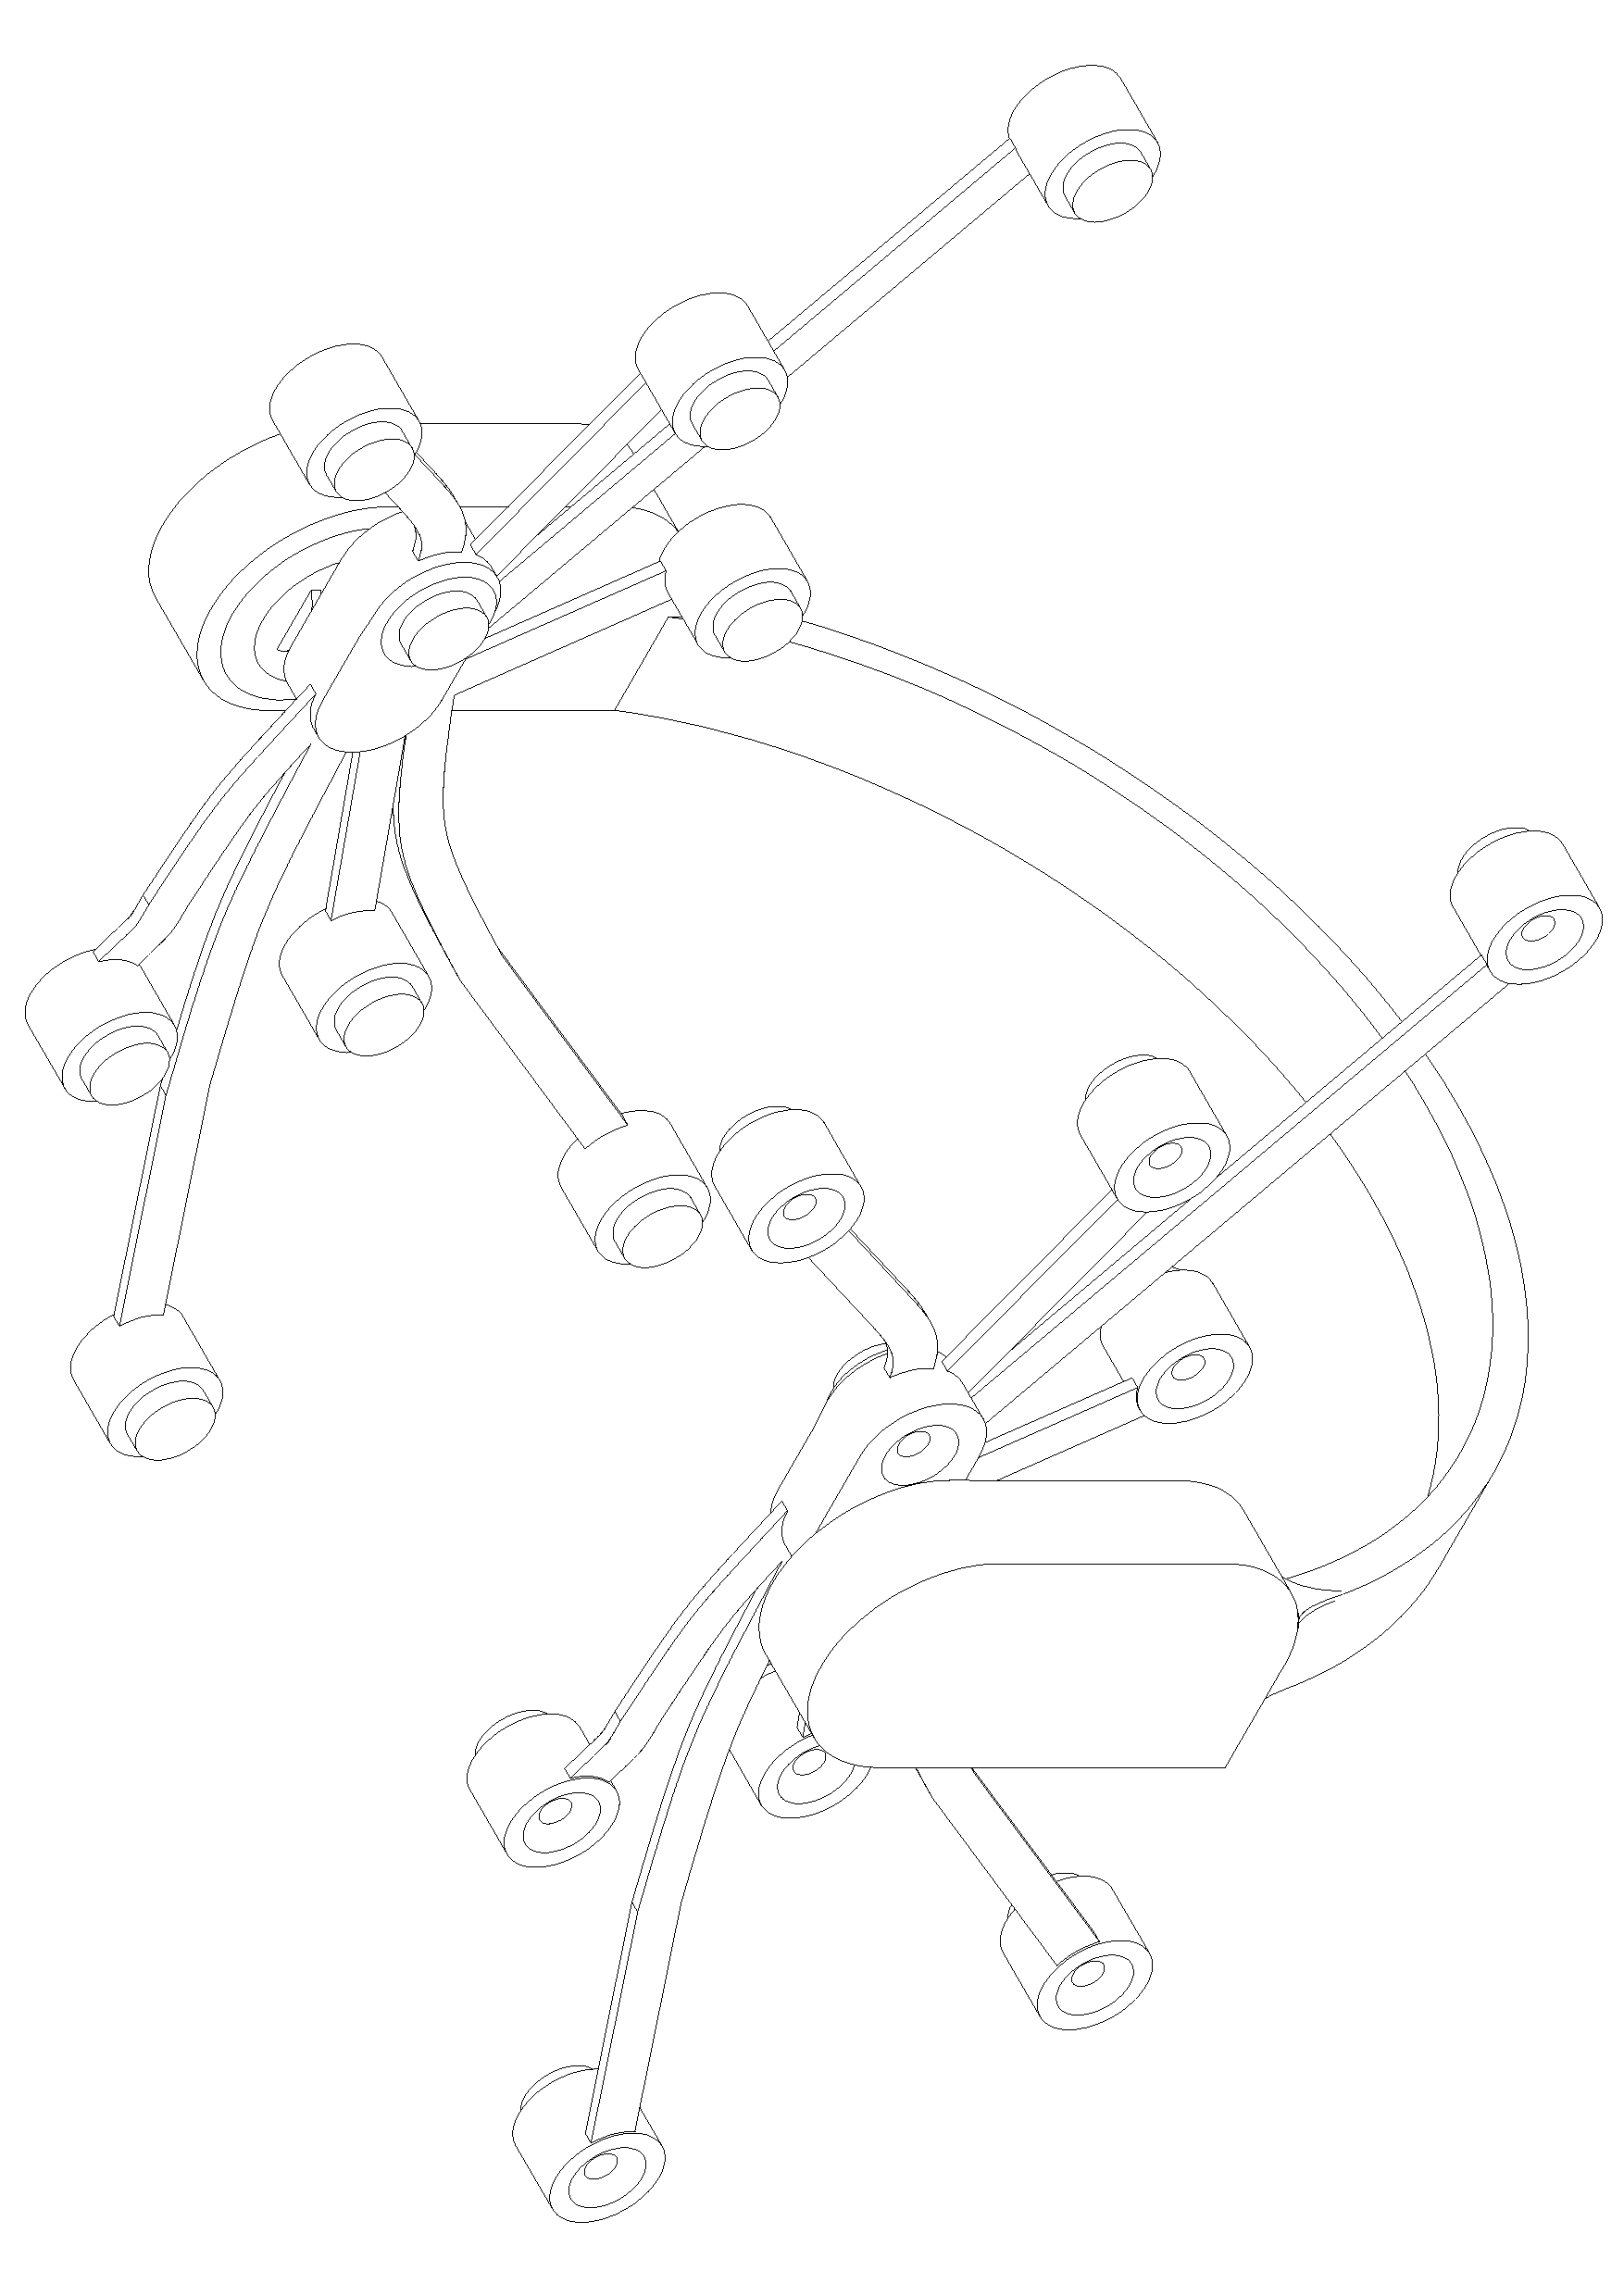
\includegraphics[angle=90,trim={14cm 0 0 0},origin=c,width=0.5\columnwidth]{./assets/yas5.pdf}
%     \caption{Położenia elektrod dla urządzenia Emotiv EPOC X}
%     \label{fig:emotiv-electrode-locations}
% \end{figure}


\begin{figure}[h!]
    \centering
    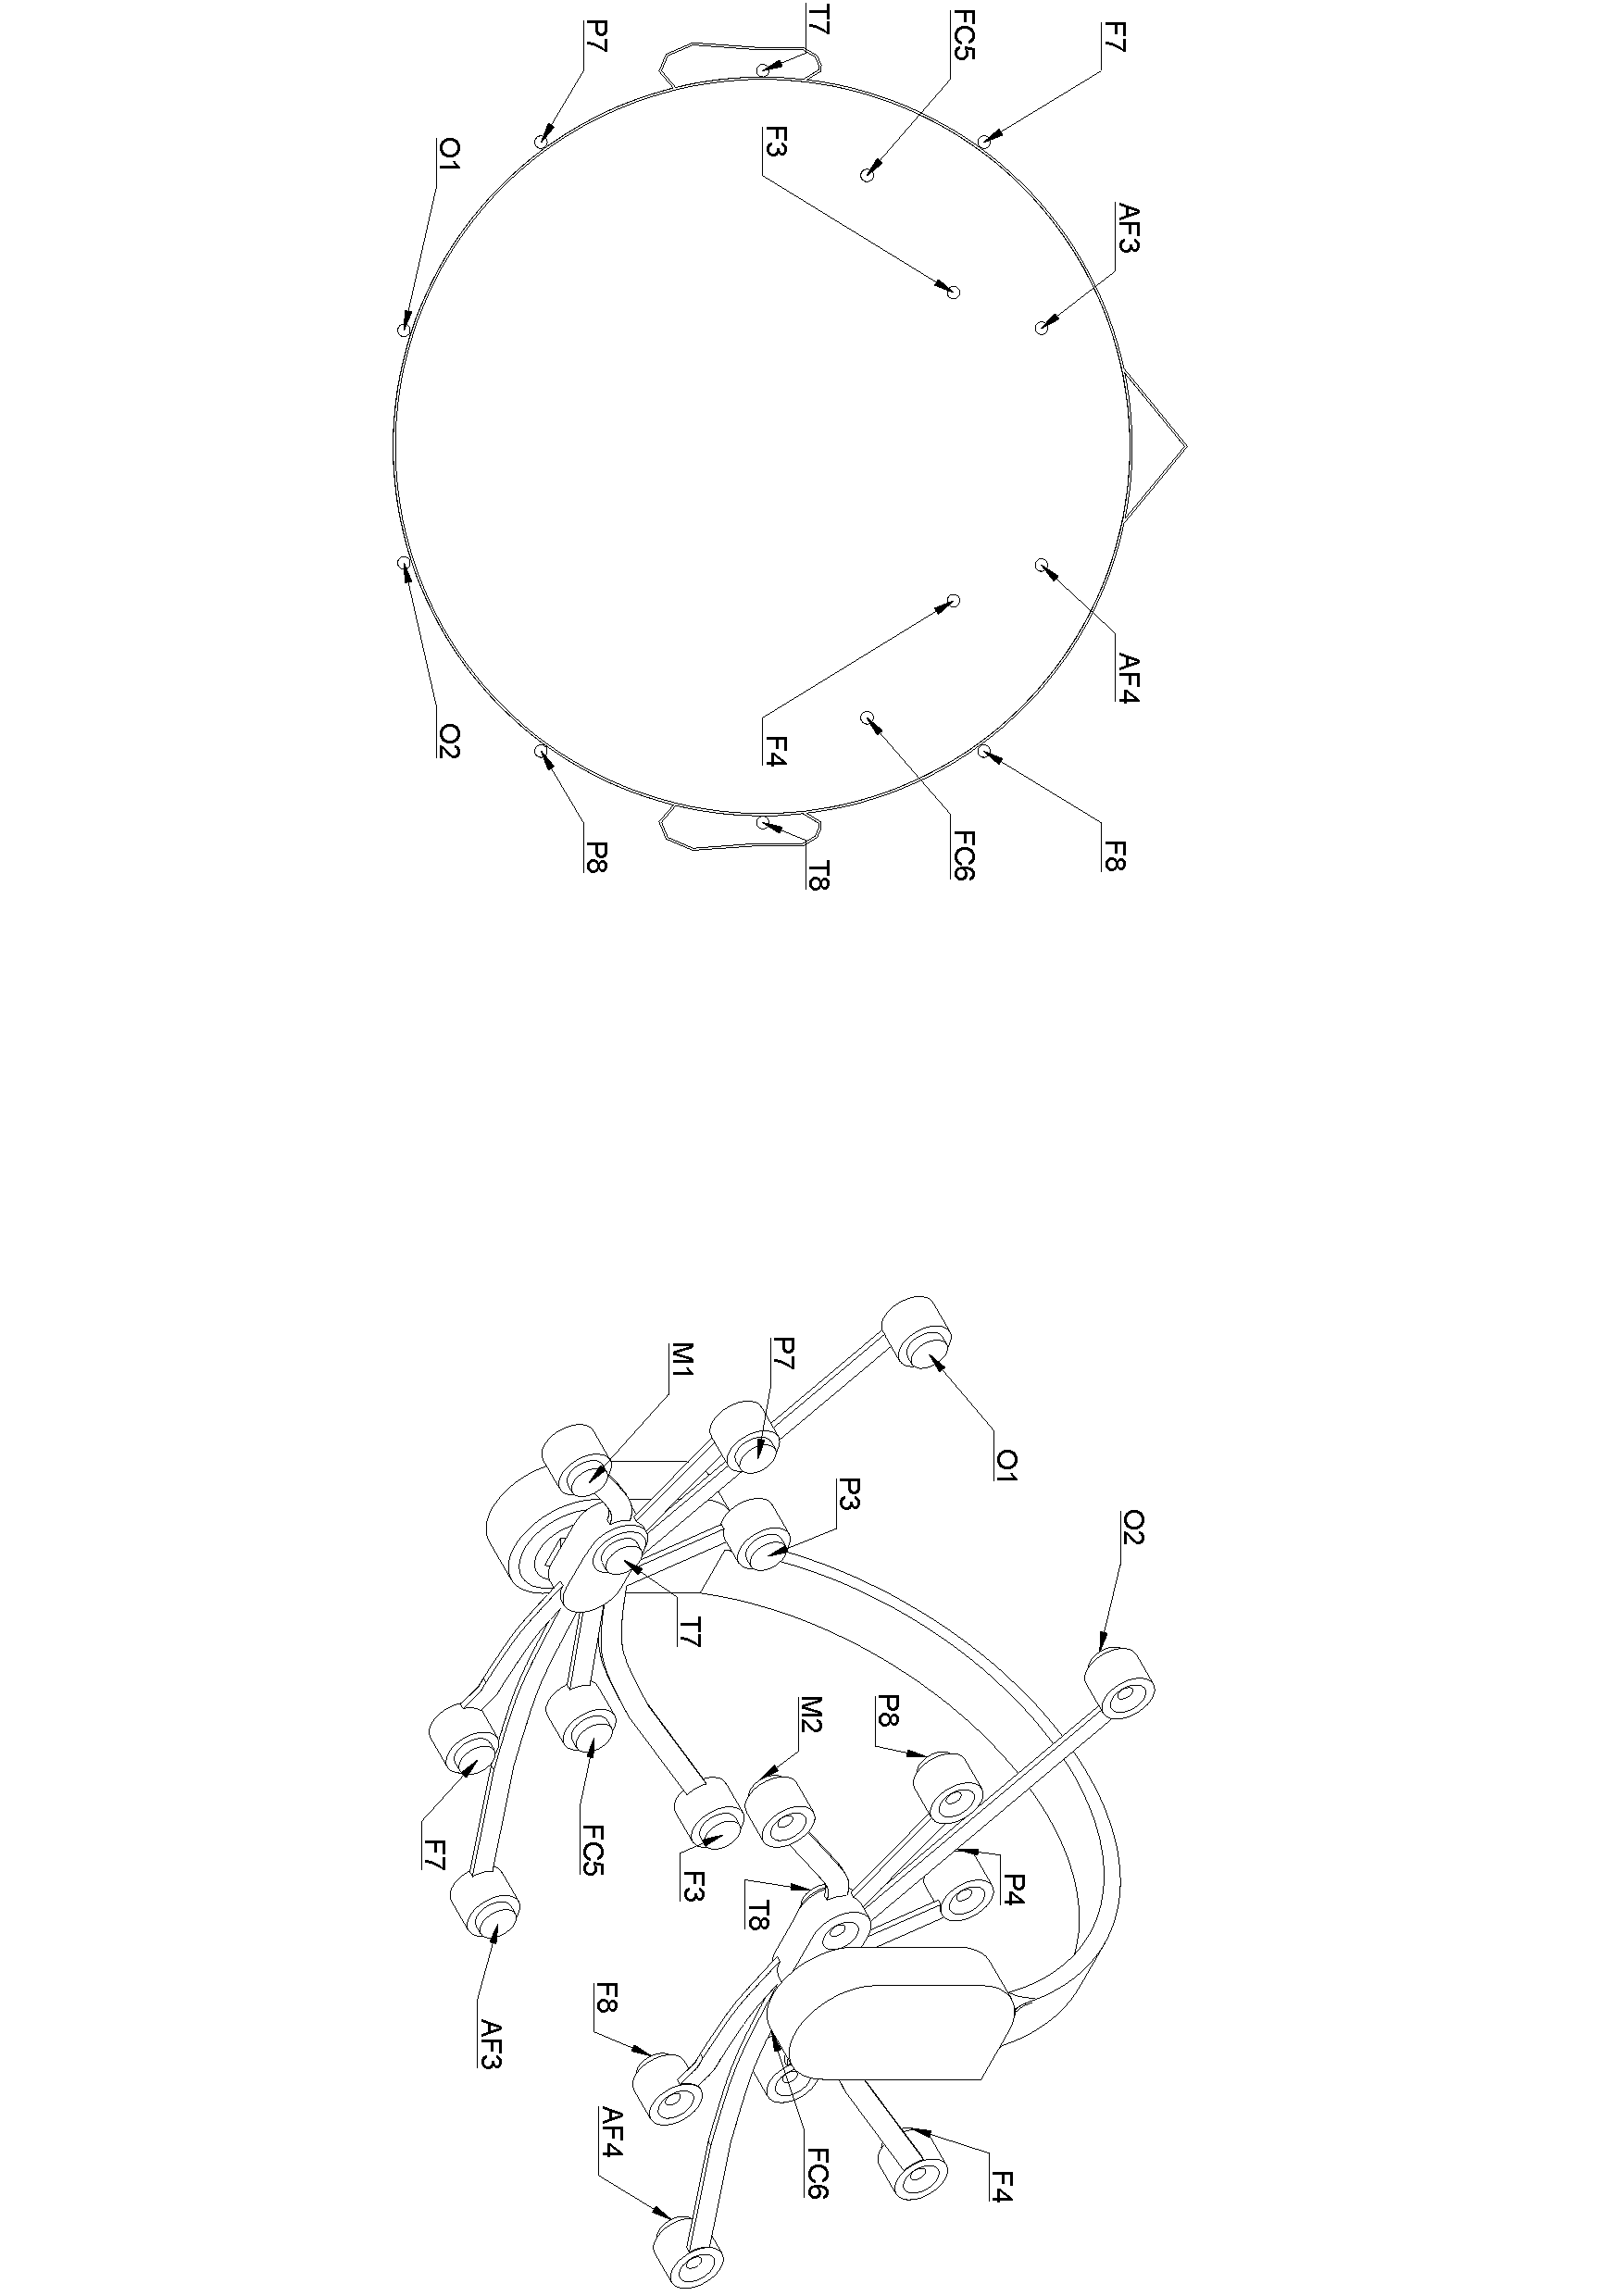
\includegraphics[angle=90,trim={35cm 0 8cm 0},origin=c,width=\columnwidth]{./assets/yas6.pdf}
    \caption{Położenia elektrod dla urządzenia Emotiv EPOC X}
    \label{fig:emotiv-electrode-locations}
\end{figure}


\section{Procedura przeprowadzonych badań}\label{procedura-badan}
% - jaki montaz
\subsection{Ankieta wejściowa}
Przed rozpoczęciem pomiarów uczestnikowi prezentowana jest ankieta wejściowa. Zawiera ona informacje na temat badania (\autoref{opis-badania}), pytania na temat okoliczności, w których ono przebiega i informacji demograficznych (\autoref{pytania-ankiety-wejsciowej}) oraz zgodę na przetwarzanie danych (\autoref{zgoda-na-przetwarzanie-danych}). Do momentu jej wyrażenia, żadne informacje nie są zapisywane.

\subsection{Przygotowanie zestawu}
Przed przystąpieniem do badania, gąbki montowane na zakończeniach elektrod zamaczane są w roztworze soli fizjologicznej, a urządzenie umieszczone zostaje na głowie badanej osoby. Jakość połączenia sprawdzana jest za pomocą oprogramowania Emotiv Pro \cite{emotiv_inc_epoc_nodate}. Po uzyskaniu zadowalającego poziomu sygnału pacjent proszony jest o zamknięcie oczu na czas około 30 sekund w celu potwierdzenia poprawnej biokalibracji (przez weryfikację występowania wzrostu aktywności w zakresie częstotliwości $\alpha$ \cite{britton_electroencephalography_2016}).

\subsection{Badanie}
Po potwierdzeniu poprawnego działania urządzenia, ochotnik zostaje zapoznany z interfejsem używanym do przeprowadzenia badania, następnie operator opuszcza pomieszczenie, a ochotnik rozpoczyna udzielanie odpowiedzi.

Badanie polega na wyświetlaniu na ekranie  serii 10 zadań arytmetycznych (\autoref{pytania-badania}). Pacjent proszony jest o wykonanie obliczeń bez wykorzystania narzędzi pomocniczych. Pytania zmieniane są automatyczne w 60-sekundowym interwale, za każdym razem w tej samej kolejności. Udzielone odpowiedzi, sygnał EEG oraz informacje o przestrzennym położeniu urządzenia są nagrywane przez cały czas trwania badania. Markery czasu wstawione zostają w momentach wyświetlenia nowego pytania i udzielenia na nie odpowiedzi.

% - https://arxiv.org/abs/1801.04503
% - https://github.com/houshd/MLSTM-FCN/blob/master/eeg2_model.py
% - sieci neuronowe
%     - rekurencyjne - motywacja stocs
% - random forest - inni ludzie
% - clustering algorithms - jako meta rozwiazanie
% - svm - inni ludzie

\chapter{Wyniki}
\section{Dostępność danych}
Dane zebrane podczas kampanii badawczej dostępne są w repozytorium projektu w surowej (po anonimizacji) i przetworzonej postaci, wraz z oprogramowaniem przygotowanym w celu ich analizy  \cite{mateusz_kojro_mateuszkojrobachelors-thesis_nodate}. 
% - publiczny dostep do zestawu dancyh
\section{Demografia}
Badaniu poddanych zostało 19 ochotników, spośród których zdecydowana większość klasuje się w przedziale od 50 do 60 ($47\%$) lub od 20 do 30 ($21\%$) lat (\autoref{fig:age}). W zbiorze zachowano balans pomiędzy ilością mężczyzn i kobiet (odpowiednio $47\%$ i $53\%$) (\autoref{fig:gender}). Większość osób badanych posiada wykształcenie wyższe ($73\%$ – rysunek \ref{fig:education}) oraz wykonuje pracę biurową ($63\%$ – rysunek \ref{fig:jobs}). Tylko jedna z badanych osób cierpi na schorzenie neurologiczne (epilepsje) w związku z czym wykonane na niej pomiary  wyeliminowane zostały ze zbioru danych.

\begin{figure}[h!]
\begin{subfigure}[b]{0.45\textwidth}
    \centering
    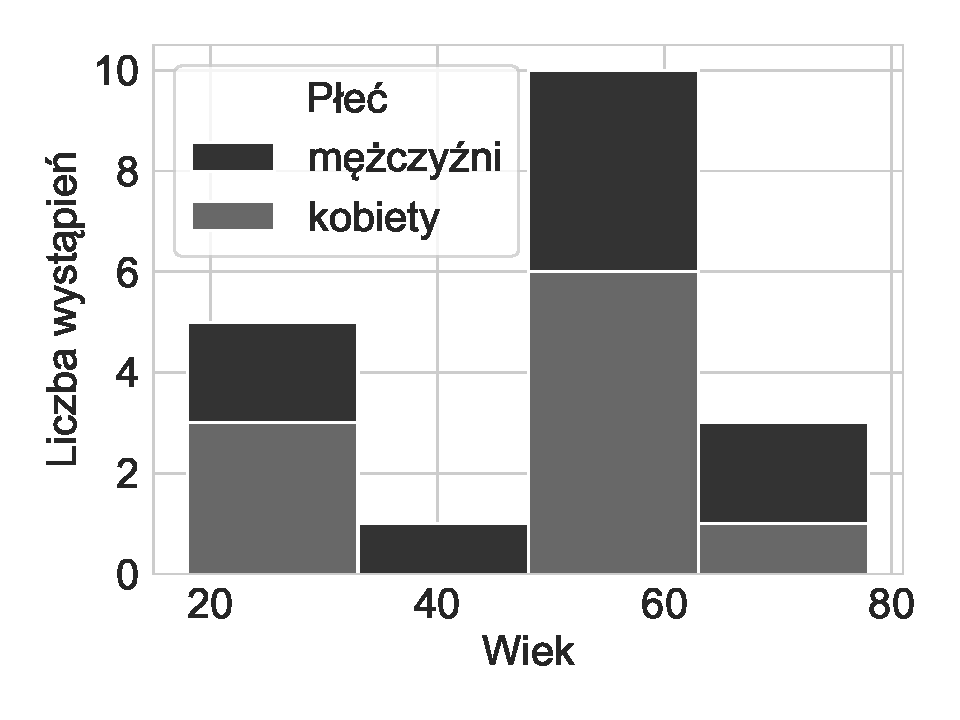
\includegraphics[width=\columnwidth]{plots/age.pdf}
    \caption{Wiek badanych osób}
    \label{fig:age}
\end{subfigure}   
\hfill
\begin{subfigure}[b]{0.45\textwidth}
    \centering
    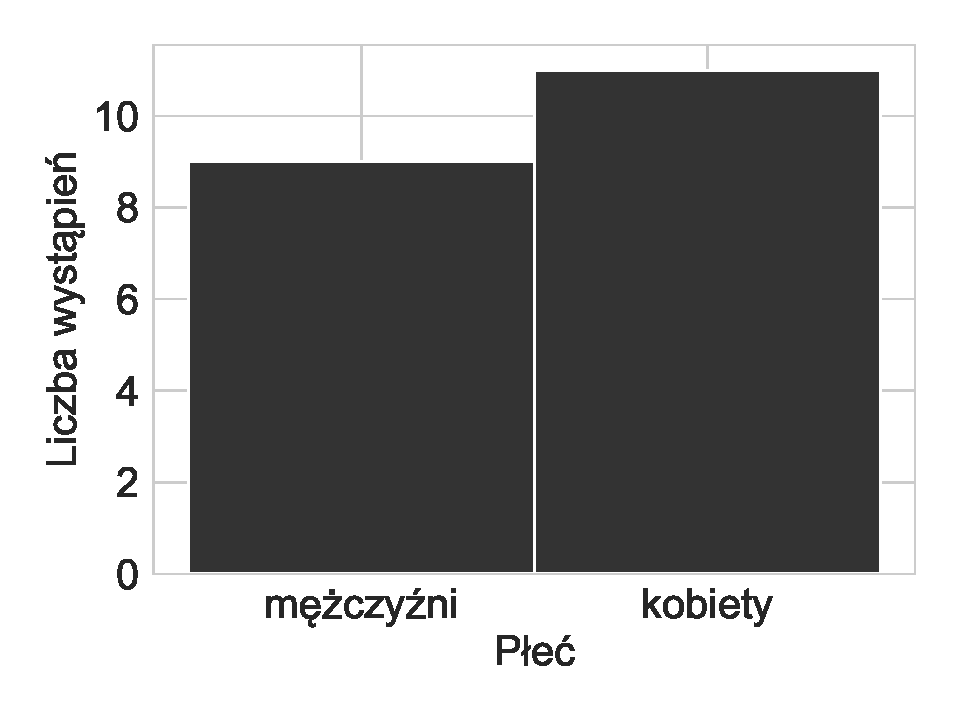
\includegraphics[width=\columnwidth]{plots/gender.pdf}
    \caption{Płeć badanych osób}
    \label{fig:gender}
\end{subfigure}
\caption{Wiek i płeć badanych osób}
\end{figure}

\begin{figure}[h!]
\begin{subfigure}[b]{0.45\textwidth}
    \centering
    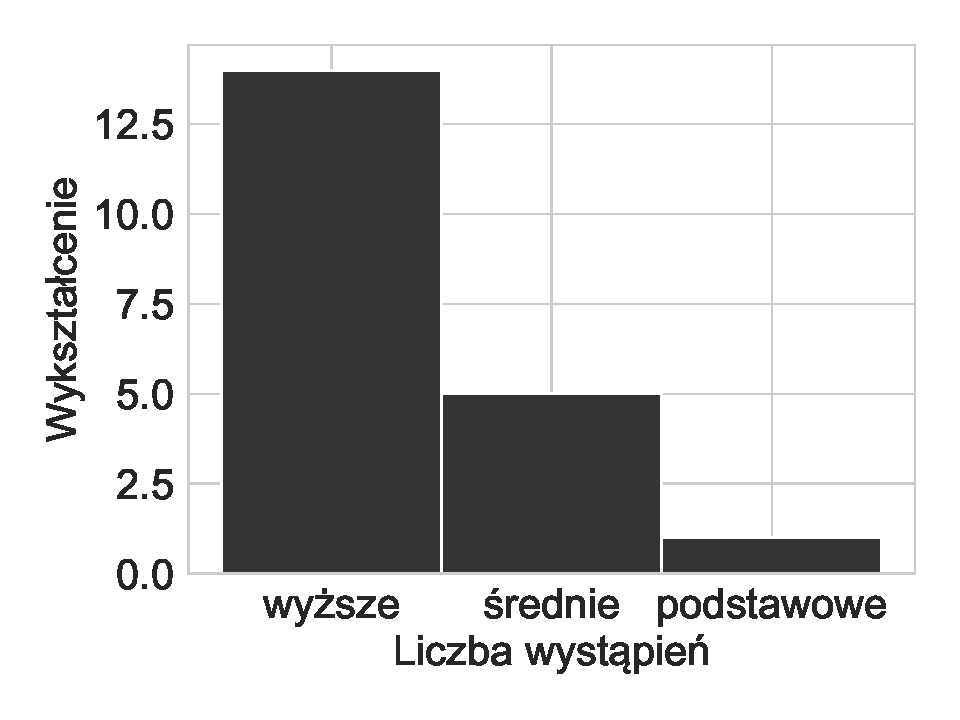
\includegraphics[width=\columnwidth]{plots/education.pdf}
    \caption{Wykształcenie}
    \label{fig:education}
\end{subfigure}   
\hfill
\begin{subfigure}[b]{0.45\textwidth}
    \centering
    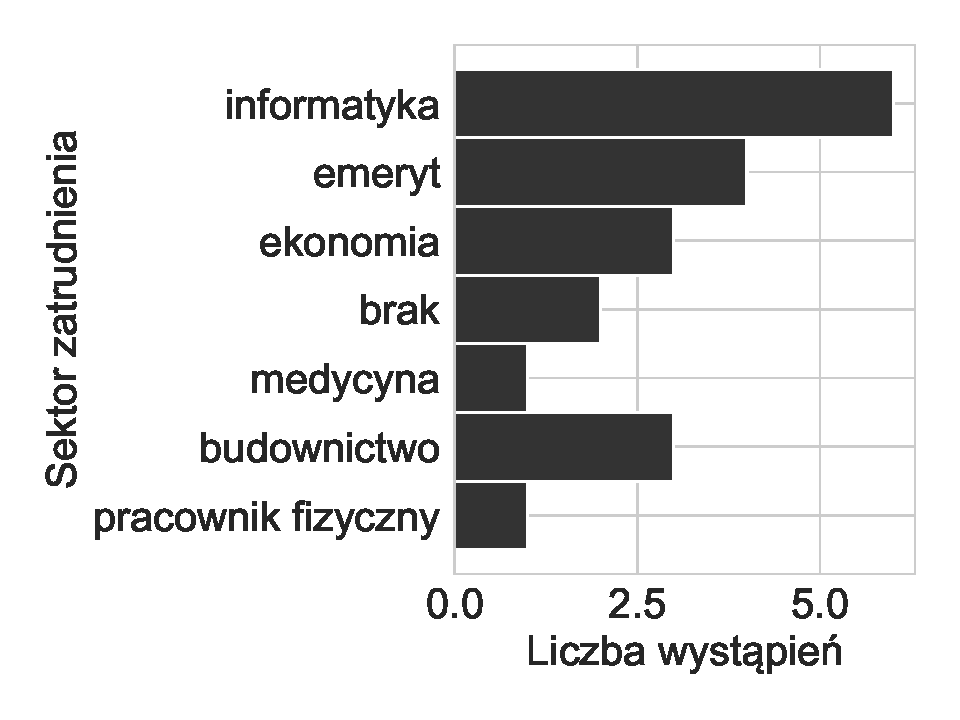
\includegraphics[width=\columnwidth]{plots/job.pdf}
    \caption{Sektor zatrudnienia}
    \label{fig:jobs}
\end{subfigure}
\caption{Wykształcenie i sektor zatrudnienia}
\end{figure}


% \begin{figure}[h!]
%     \centering
%     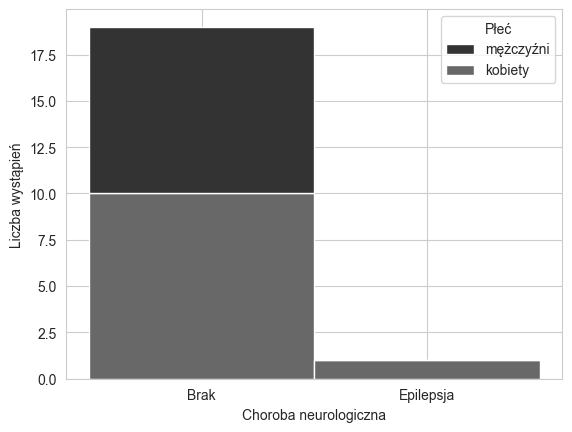
\includegraphics[width=0.5\columnwidth]{thesis/assets/neurological_disease.png}
%     \caption{Choroby neurologiczne badanych osób}
%     \label{fig:neurological-diseses}
% \end{figure}

% Sprawdzanie tezy ze kazda z tych zmiennych opisuje wyniki
% - Wiek
% - Płeć
% - Wykształcenie
% - Zawód
% - Choroby neurologiczne/psychologiczne
% - Stopien zaznajomienia z komputerami
\section{Przygotowanie zbioru danych}\label{data-preparation}

W pierwszym kroku zebrane dane poddane zostały procesowi anonimizacji, imiona, nazwiska i adresy email zostały usunięte, a
daty urodzenia zamieniono na przedziały wieku. Następnie w celu eliminacji obserwacji odstających wykorzystano tzw. ,,metrykę $Z$'' (ang. \textit{zscore}) \cite{noauthor_scipystatszscore_nodate}, obliczaną z pomocą równania \ref{eq:zscore} w którym $x$ oznacza wartość zmiennej, $\mu$ średnią populacji, a $\sigma$ jej odchylenie standardowe. Poziom odrzucenia ustalono na $z=3$. Metryka ta zaaplikowana została do średniego potencjału zmierzonego na każdej z elektrod (listing \ref{lst:z-score-calculation} zawiera implementację tej operacji z wykorzystaniem bibliotek NumPy \cite{harris_array_2020} i SciPy \cite{virtanen_scipy_2020}). Spośród wykonanych pomiarów tylko jeden (osoba Q) przekroczył poziom odrzucenia, w związku z czym został wyeliminowany z dalszej analizy. Rysunek \ref{fig:zscore} prezentuje wyniki obliczeń.

\begin{equation}
    z = \frac{x - \mu}{\sigma}
\end{equation}\label{eq:zscore}

\begin{lstlisting}[caption={Obliczanie standardyzacji Z},label={lst:z-score-calculation}]
import numpy as np
from scipy.stats import zscore

# X zawiera wszystkie probki zebrane na wszystkich kanalach
# X.shape = (liczba probek, liczba osob, liczba kanalow)
zscores = np.abs(zscore(X)).max(axis=1)
\end{lstlisting}

\begin{figure}[h!]
    \centering
    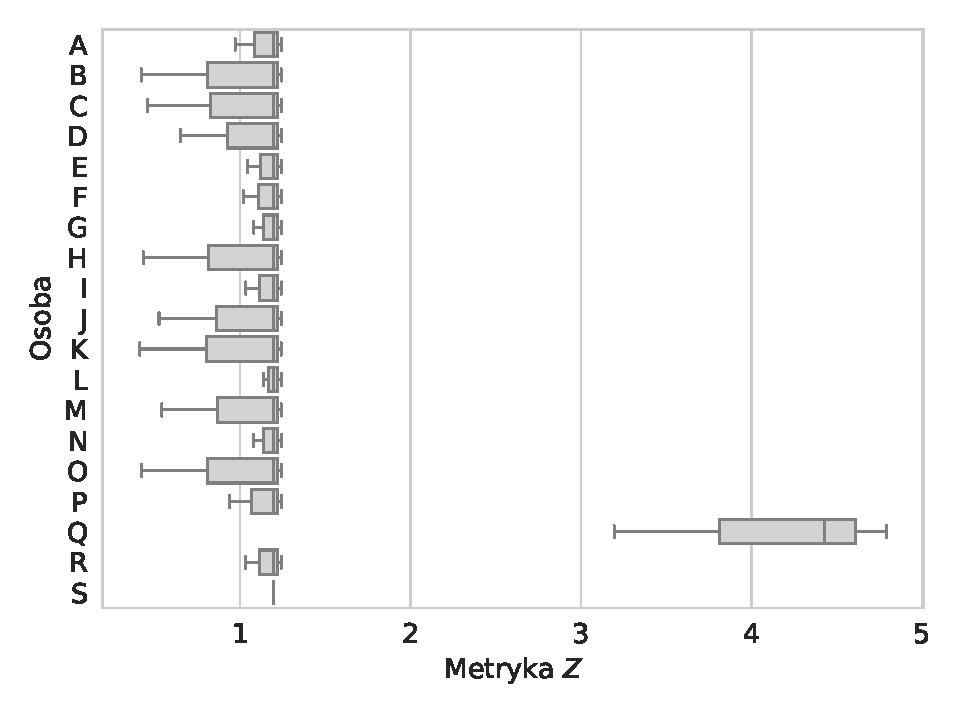
\includegraphics[width=0.75\columnwidth]{plots/zscore.pdf}
    \caption{Wartości metryki $Z$}
    \label{fig:zscore}
\end{figure}

Pozostałe dane zostały pogrupowane ze względu na wykonywaną aktywność – czas od wyświetlenia pytania do udzielenia odpowiedzi zakwalifikowany został jako stan skupienia ($t_f$), a czas pozostały do wyświetlenia kolejnego zadania przyjęto jako stan spoczynku – $t_r$ (czas kalibracji, $t_c$, został oddzielony od poprzednich grup). 
Przygotowano również pochodny zbiór danych stworzony poprzez aplikację do zebranych pomiarów dyskretnej transformaty Fouriera (rozmiar okna wybrano na $128$ próbek – jedną sekundę pomiaru).  Średnie wartości dla częstotliwości najczęściej badanych w środowisku medycznym przedstawiono na rysunkach \ref{fig:waiting}, \ref{fig:thinking} i \ref{fig:diff} (odpowiednio czas spoczynku, skupienia i różnica między nimi).

\begin{figure}[h!]
    \centering
    \begin{subfigure}[b]{\textwidth}
    \centering
    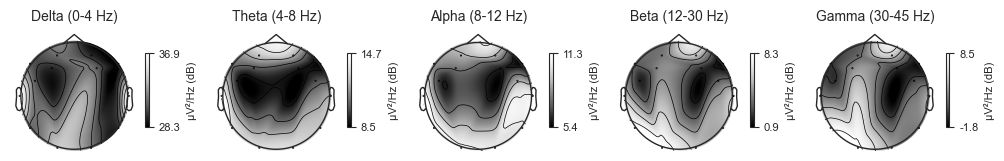
\includegraphics[width=\columnwidth]{thesis/assets/waiting.png}
    \caption{Aktywność mózgu w czasie oczekiwania}
    \label{fig:waiting}
\end{subfigure}


\begin{subfigure}[b]{\textwidth}
    \centering
    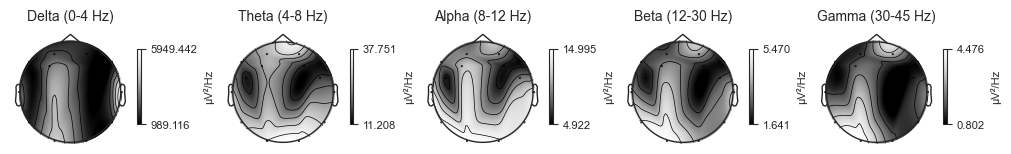
\includegraphics[width=\columnwidth]{thesis/assets/thinking.png}
    \caption{Aktywność mózgu w czasie wykonywania zadania}
    \label{fig:thinking}
\end{subfigure}


\begin{subfigure}[b]{\textwidth}
    \centering
    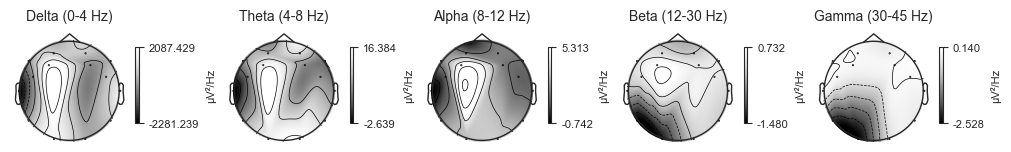
\includegraphics[width=\columnwidth]{thesis/assets/diff.png}
    \caption{Różnica pomiędzy aktywnością mózgu w czasie myślenia i w czasie oczekiwania}
    \label{fig:diff}
\end{subfigure}
    \includegraphics[width=0.5\columnwidth]{}
    \caption{Porównanie siły poszczególnych częstotliwości w różnych punktach na czaszce}
    \label{fig:brain-heatmaps}
\end{figure}

\section{Analiza statystyczna}\label{analiza-klasyczna}
W celu udowodnienia różnicy pomiędzy zmierzoną aktywnością mózgu w czasie skupienia i w czasie spoczynku średnie częstotliwości zmierzone na każdej z elektrod porównane zostały za pomocą testu Kruskala \cite{noauthor_scipystatskruskal_nodate}. Poziom istotności statystycznej przyjęto na $\alpha=0,95$. Rysunek \ref{fig:thinking-vs-waiting-pvalue} przedstawia obliczone wartości $p$, sugerujące statystycznie znaczące różnice dla niektórych kombinacji kanałów i zakresów częstotliwości (przedziały zgodne z podanymi w tabeli \ref{tab:freqs}).
\begin{figure}[h!]
    \centering
    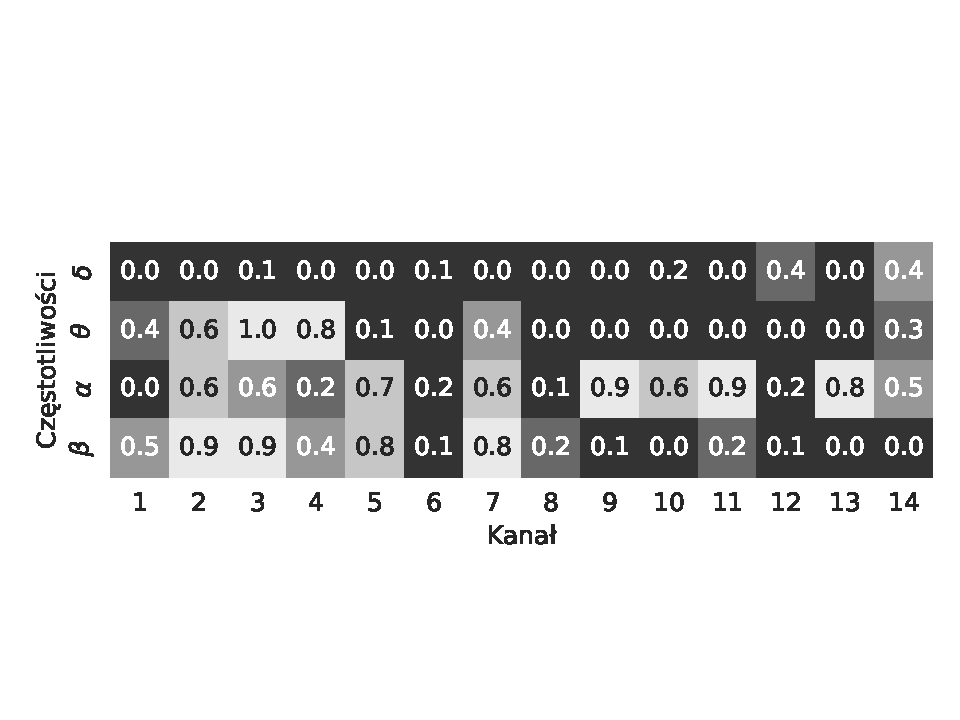
\includegraphics[width=\columnwidth,trim={0 2.9cm 0 4cm}, clip]{plots/pvalue.pdf}
    \caption{Porównanie wartośći $p$ dla różnych zakresów częstotliwości i kanałów}
    \label{fig:thinking-vs-waiting-pvalue}
\end{figure}
% \begin{lstlisting}[caption={Przejście do domeny częstotliwościowej},label={lst:moving-to-freq-domain}]
% import numpy as np
% from scipy.fft import fft
% # X zawiera wszystkie probki zebrane na wszystkich kanalach
% # X.shape = (liczba probek, liczba kanalow)
% X = X.reshape(-1, num_channels, window_size)
% freq_domain = np.abs(fft(X, axis=-1))
% deltas = np.sum(freq_domain[:, :, 1:3], axis=-1)
% thetas = np.sum(freq_domain[:, :, 4:7], axis=-1)
% alphas = np.sum(freq_domain[:, :, 8:13], axis=-1)
% betas = np.sum(freq_domain[:, :, 14:25], axis=-1)
% \end{lstlisting}

\subsection{Zmienne zakłócające}\label{zmiennne-zaklucajace}
Ankieta wstępna wypełniania przez pacjentów zawierała pytania mające na celu ocenę czynników, które mogłyby wpłynąć na wyniki badania, takich jak ilość czasu spędzonego przy komputerze (\autoref{fig:computer-time}), godziny snu poprzedniej nocy (\autoref{fig:sleep-time}), poziom zmęczenia (\autoref{fig:tired}), przyjmowane substancje psychoaktywne (\autoref{fig:psychoactive-substances}) oraz częstotliwość wykonywania mentalnych obliczeń arytmetycznych (\autoref{fig:arithmetic}).

\begin{figure}[h!]
\begin{subfigure}[b]{0.45\textwidth}
    \centering
    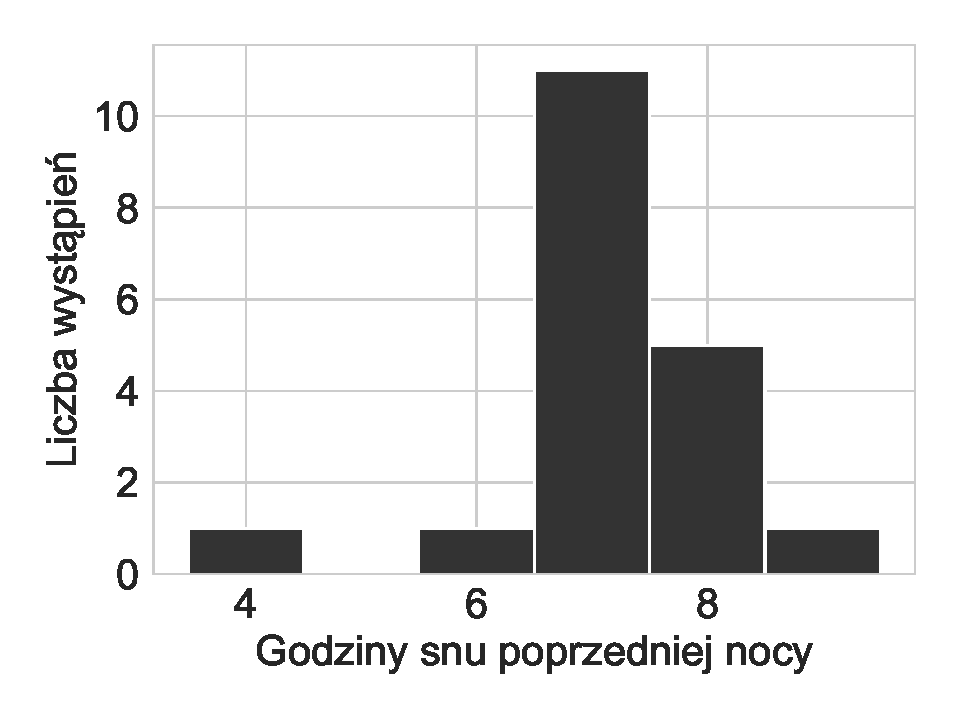
\includegraphics[width=\columnwidth]{thesis/plots/sleep.pdf}
    \caption{Godziny snu poprzedniej nocy}
    \label{fig:sleep-time}
\end{subfigure}   
\hfill
\begin{subfigure}[b]{0.45\textwidth}
    \centering
    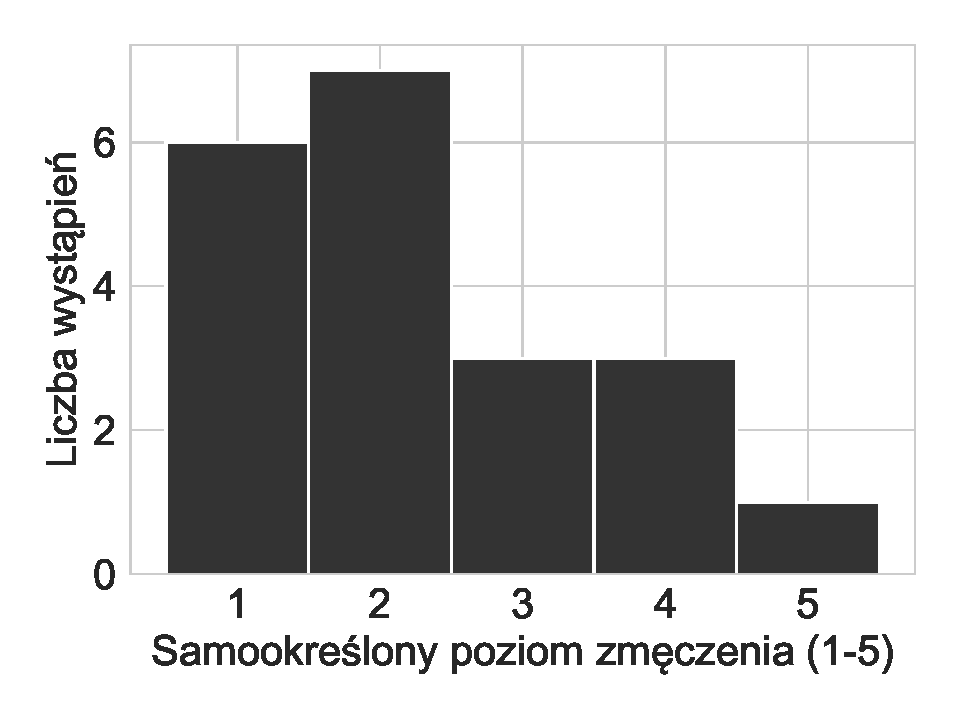
\includegraphics[width=\columnwidth]{thesis/plots/exhaustion_level.pdf}
    \caption{Samookreślony poziom zmęczenia}
    \label{fig:tired}
\end{subfigure}
\begin{subfigure}[b]{0.45\textwidth}
    \centering
    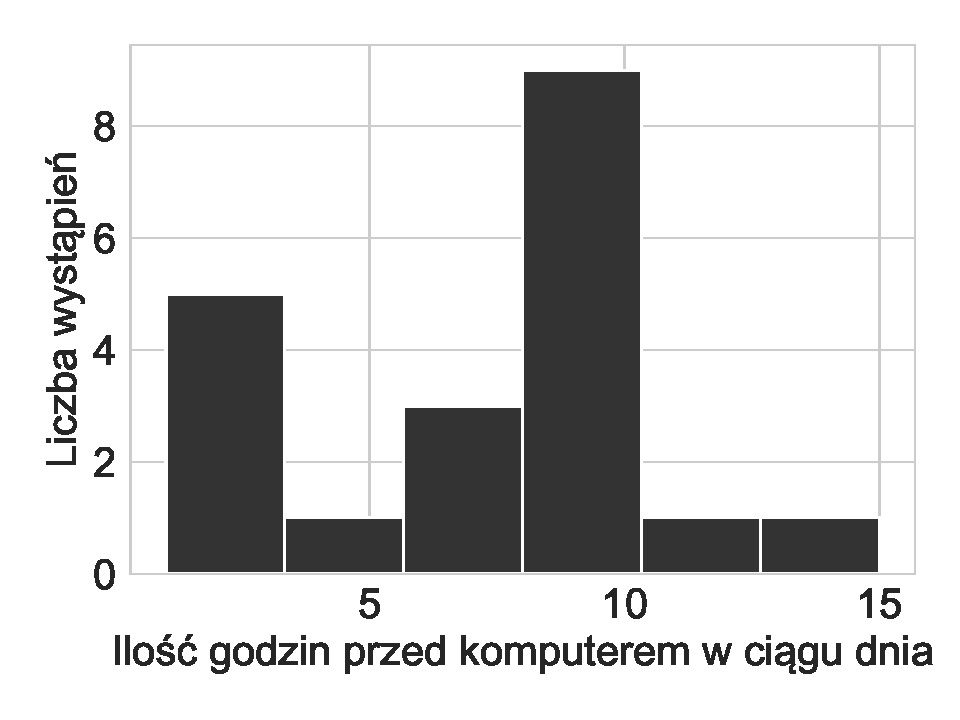
\includegraphics[width=\columnwidth]{thesis/plots/computer_hours.pdf}
    \caption{Czas spędzany przy komputerze w ciągu dnia}
    \label{fig:computer-time}
\end{subfigure}   
\hfill
\begin{subfigure}[b]{0.45\textwidth}
    \centering
    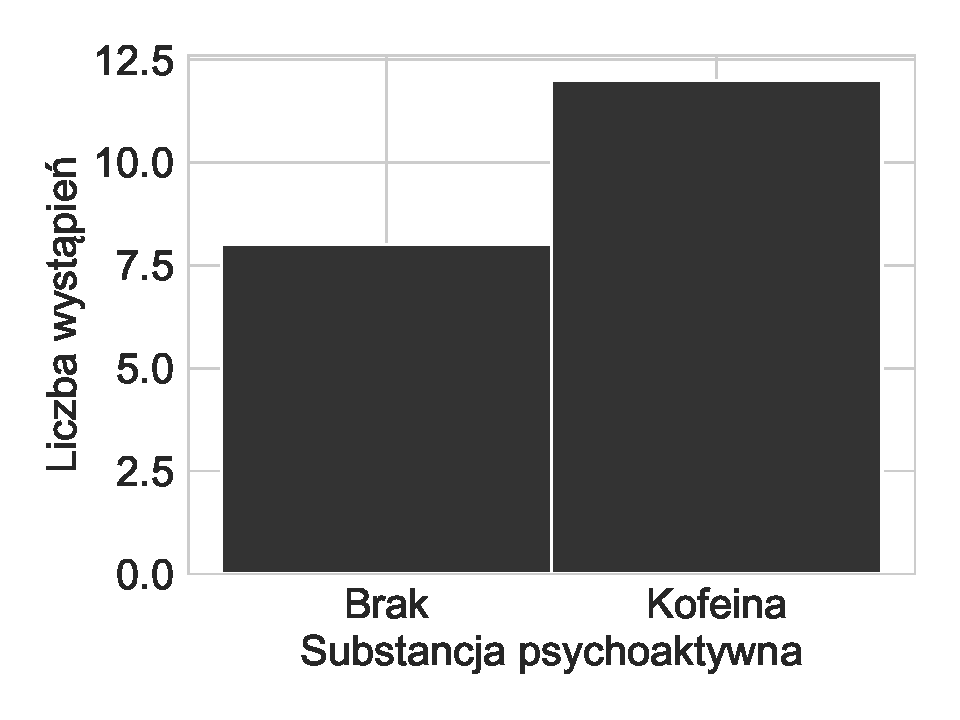
\includegraphics[width=\columnwidth]{thesis/plots/psychoactive_substances.pdf}
    \caption{Substancje psychoaktywne przyjętę w ciągu 6 godzin przed rozpoczęciem badania}
    \label{fig:psychoactive-substances}
\end{subfigure}
\begin{subfigure}[b]{\textwidth}
\centering
    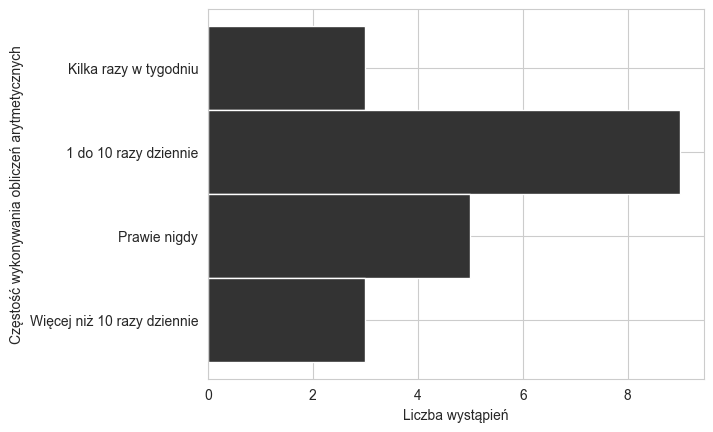
\includegraphics[width=0.75\columnwidth]{thesis/assets/mental_math.png}
    \caption{Histogram samookreślonej częstotliwości wykonywania mentalnych obliczeń arytmetycznych}
    \label{fig:arithmetic}
\end{subfigure}
\caption{Histogramy dla zmiennych zakłócających}
\end{figure}

W celu określenia wpływu badanych zmiennych zakłócających na wykonane pomiary każdą zmienną podzielono na dwa przedziały wysoki i niski. Następnie zastosowano jednoczynnikową analizę wariacji (ang \textit{one-way ANOVA}) w celu sprawdzenia statystycznie istotnej różnicy pomiędzy nimi (przyjęto poziom istotności wysokości $\alpha=0,95$), a wyniki przedstawiono w tabeli \ref{tab:confunding-variables-statistical-tests} 

\begin{table}[h!]
    \centering
    \begin{tabular}{|c|c|c|}
        \hline
          Zmienna zakłócająca & Wartość $p$\\
        \hline
         Płeć & $0,06 $\\
         Mniej niż $8$ godzin snu & $<0,01$ \\
         Substancje psychoaktywne  & $<0,01$ \\
         Samookreślony poziom zmęczenia większy niż $3$ & $<0,01$ \\
         Czas spędzany przy komputerze dłuższy niż 8 godzin & $<0,01$ \\
         Częste wykonywanie mentalnych obliczeń \footnotemark & $<0,01$ \\
         Poziom naładowania baterii poniżej $50\%$ & $<0,01$ \\
        \hline
    \end{tabular}
    \caption{Wyniki testów statystycznych na różnice w sygnale pomiędzy różnymi wartościami zmiennych zakłócających}
    \label{tab:confunding-variables-statistical-tests}
\end{table}
\footnotetext{Odpowiedzi \textit{1-10 razy dziennie} i \textit{Więcej niż 10 razy dziennie}}

% \subsection{Outlier detection}
% \subsection{ANOVA}
% \subsection{Fourier}
% - roznica u osoby z epilepsja 
% - odseparowac momenty wyswietlenia pytania i udzielenia odpowiedzi i porownac z stanem domyslnym
% - porownac czestotliwosci na poczatku badania i na koncu
% - interesujace korelacje z innymi zmiennymi (maybe macierz korelacji)
\section{Uczenie maszynowe}\label{uczenie-maszynowe}
\subsection{Transformacje danych i architektura sieci}
W celu opracowania algorytmu wykrywania stanu skupienia przetestowano szereg różnego rodzaju algorytmów uczenia maszynowego, między innymi lasy losowe, gęste i konwolucyjne sieci neuronowe oraz specjalistyczne sieci do klasyfikacji szeregów czasowych (wykorzystujące architekturę MLSTM-FCN \cite{karim_multivariate_2019}). Na rysunku \ref{fig:arch} przedstawiono architekturę zaimplementowanych modeli. Wymiary warstw umieszczone zostały w nawiasach, gdzie pierwsza wartość oznacza rozmiar wejścia, druga rozmiar wyjścia a opcjonalna trzecia wymiary filtra (przy splotach dwuwymiarowych stosowano filtry kwadratowe), symbolem $X$ oznaczono wymiary zależne od kształtu wejścia.

Zestawy danych przygotowane w sekcji \ref{data-preparation} znormalizowane zostały przez usunięcie średniej i przeskalowanie do odchylenia standardowego, a następnie podzielone na próbki czasowe o rozmiarach od $1$ do $256$ kroków czasowych. Wpływ rozmiaru okna na uczenie modelu sprawdzony został, poprzez trenowanie lasu losowego na tym samym zbiorze pomiarów z różnym rozmiarem okna czasowego jako wejścia (\autoref{fig:window-size}).

\begin{figure}
    \centering
    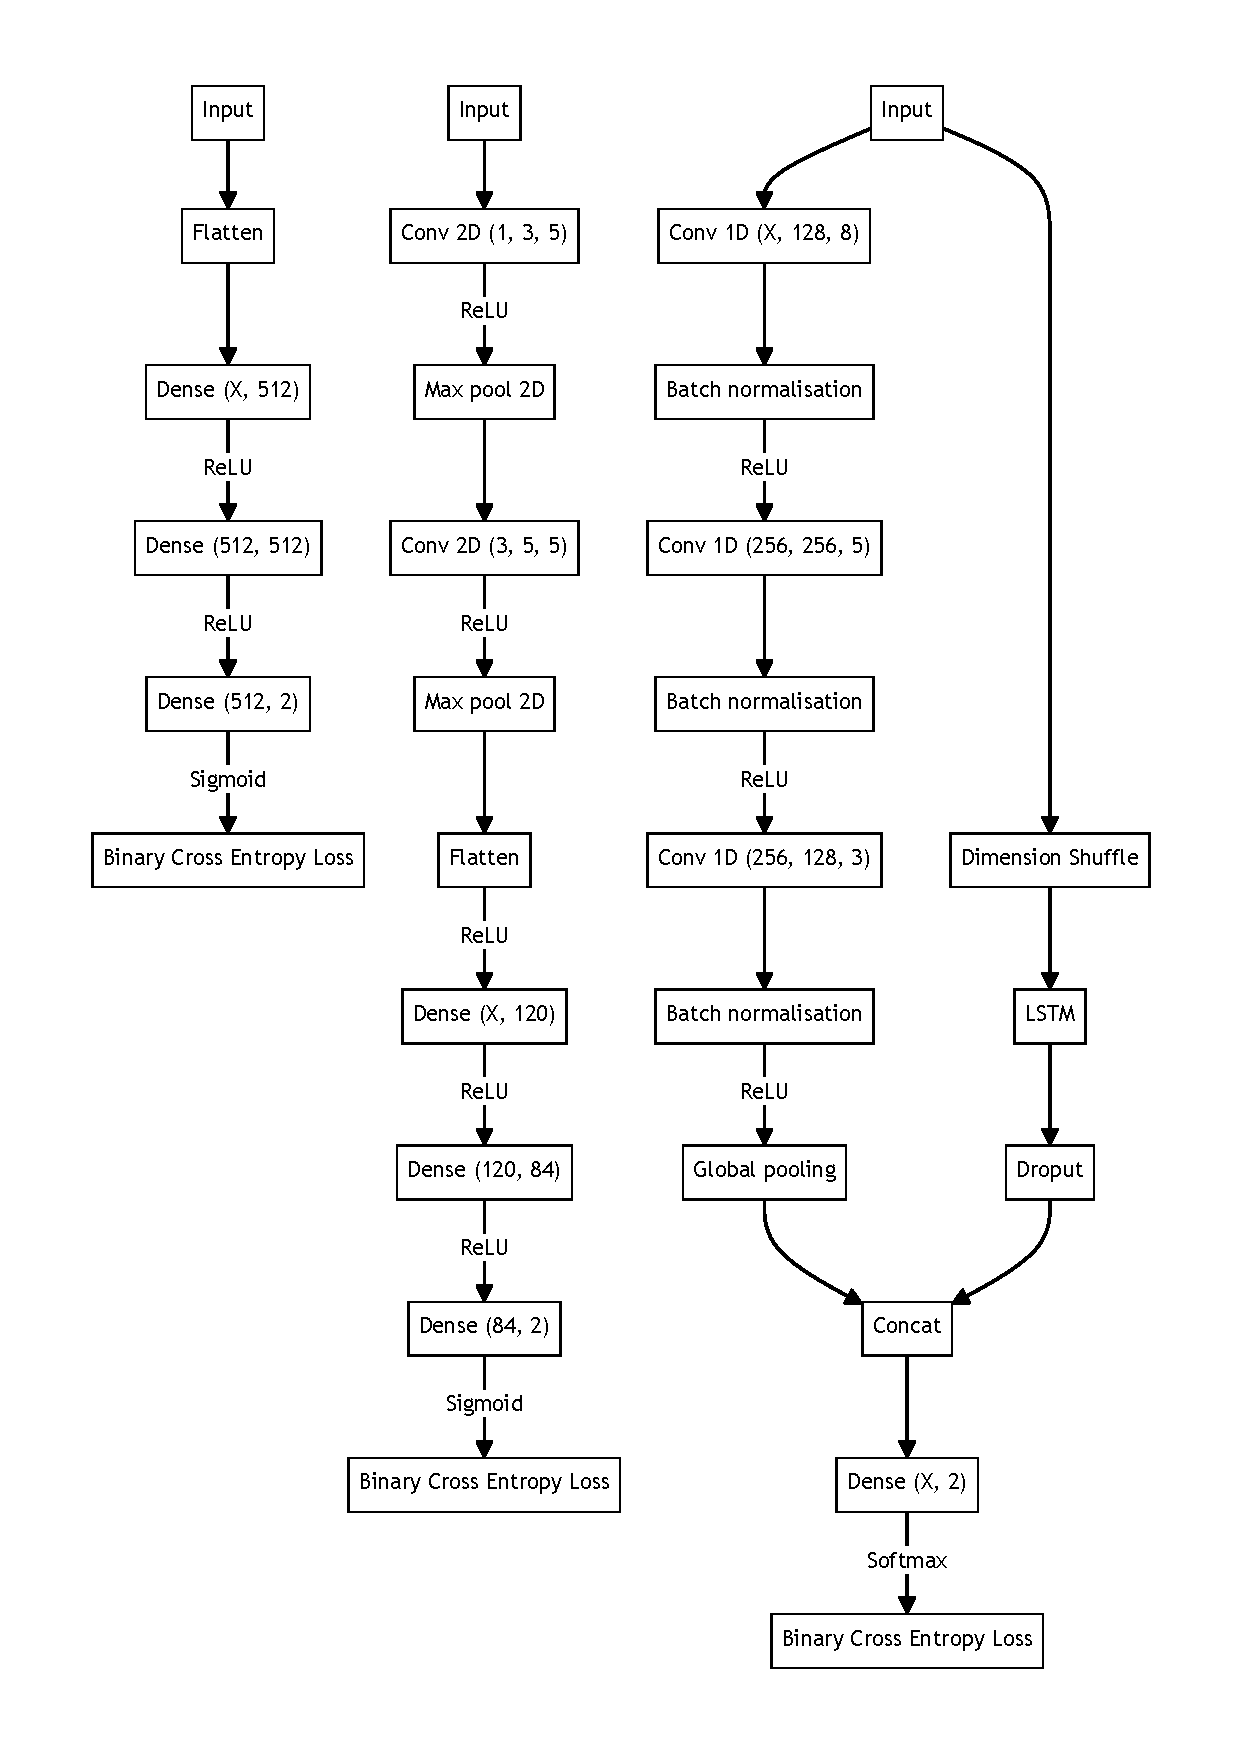
\includegraphics[width=\columnwidth]{diagrams/network_arch.pdf}
    \caption[Schematy architektury zaimplementowanych sieci neuronowych]{Schematy architektury zaimplementowanych sieci neuronowych – sieć gęsta (lewo), konwolucyjna (środek) oraz MLSTM (prawo)}
    \label{fig:arch}
\end{figure}

\begin{figure}[h!]
    \centering
    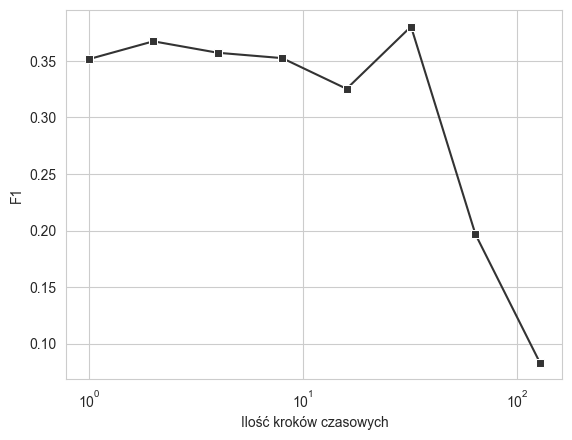
\includegraphics[width=0.5\columnwidth]{thesis/assets/window_size_vs_f1.png}
    \caption{Porównanie miary $F_1$ dla lasu losowego, na zbiorze walidacyjnym ze względu na wielkość okna czasowego}
    \label{fig:window-size}
\end{figure}

Zestaw danych walidacyjnych przygotowany został poprzez oddzielenie pomiarów wykonanych na trzech osobach i niewykorzystywanie go podczas trenowania algorytmów. Do oceny jakości modelu stosowana jest standardowa dla problemów klasyfikacji binarnej miara F1 (obliczana za pomocą wzoru \ref{eq:calculation-f1}) oraz dokładność (wzór \ref{eq:accuracy}).

\begin{equation}\label{eq:calculation-f1}
    F_1 = \frac{2*\text{prawdziwie pozytywne}}{2*\text{prawdziwie pozytywne}+\text{fałszywie pozytywne}+\text{fałszywie negatywne}}
\end{equation}

\begin{equation}\label{eq:accuracy}
    A_{cc} = \frac{\text{prawdziwie pozytywne} + \text{prawdziwie negatywne}}{\text{wszystkie próbki}}
\end{equation}

\subsection{Przeprowadzone eksperymenty i rezultaty}
W celu dobrania odpowiednich metod opracowania danych oraz wartości hiperparametrów przygotowywanych modeli przeprowadzono eksperymenty mające na celu ich ustalenie. Modele trenowane były wykorzystując strategię optymalizacji Adam \cite{kingma_adam_2017} przez minimum 500 epok. Metryki $F_1$ oraz $A_{cc}$ obliczane były na zbiorze walidacyjnym po ukończeniu każdej z nich, a najlepsze uzyskane wartości przedstawiono w tabeli \ref{tab:high-level-results} jednoznacznie pokazując brak zdolności predykcyjnej uzyskanych algorytmów.

% Natomiast głębokość lasu losowego dostosowana została przez jej sukcesywne zwiększanie aż do osiągnięcia stabilizacji (\autoref{fig:rf-num-nodes}).


% \begin{figure}[h!]
%     \centering
%     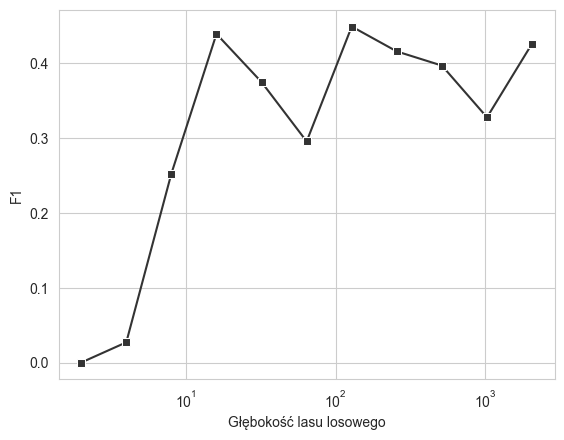
\includegraphics[width=0.5\columnwidth]{thesis/assets/forest_depth_vs_f1.png}
%     \caption{Porównanie miary $F_1$ na zbiorze walidacyjnym z względu na ilość warstw lasu losowego}
%     \label{fig:rf-num-nodes}
% \end{figure}

% \begin{figure}[h!]
%     \centering
%     \includegraphics[width=0.5\columnwidth]{}
%     \caption{Porównanie miary F1 na zbiorze walidacyjnym z rozmiar okna średniej ruchomej}
%     \label{fig:rolling-average-window-size}
% \end{figure}

\begin{table}[h]
    \centering
    \begin{tabular}{|c|c|c|}
        \hline
                 & Napięcia na elektordach & Częstotliwośći na elektrodach  \\
        \hline
        Las losowy &  &  \\
        Sieć gęsta &  & $0,74$ ($0,64$) \\
        Sieć konwolucyjna & & $0,70$ ($0,60$) \\
        Sieć MLSTM & & \\
        \hline
    \end{tabular}
    \caption{Najlepsze wyniki miary $F_1$ oraz $A_{cc}$ na zbiorze walidacyjnym z podziałem na rodzaj modelu i rodzaj danych wejściowych}
    \label{tab:high-level-results}
\end{table}



% \begin{figure}[h!]
%     \centering
%     \begin{subfigure}[b]{0.45\textwidth}
%         \centering
%         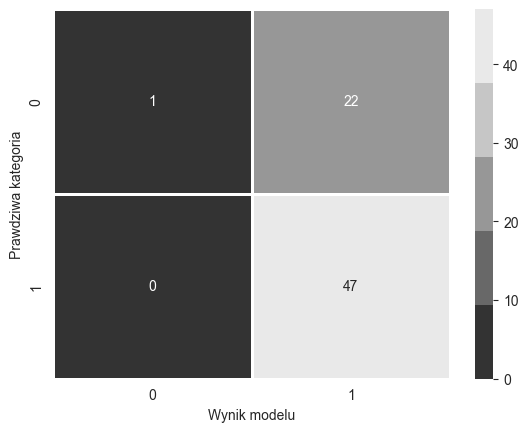
\includegraphics[width=\columnwidth]{thesis/assets/confusion_matrix_placeholder.png}
%         \caption{Las losowy – Napięcia}
%         \label{fig:computer-time}
%     \end{subfigure}   
%     \hfill
%     \begin{subfigure}[b]{0.45\textwidth}
%         \centering
%         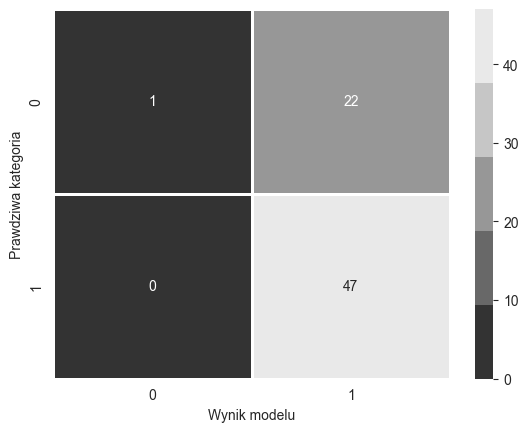
\includegraphics[width=\columnwidth]{thesis/assets/confusion_matrix_placeholder.png}
%         \caption{Las losowy – Częstotliwości}
%         \label{fig:psychoactive-substances}
%     \end{subfigure}
%     \begin{subfigure}[b]{0.45\textwidth}
%         \centering
%         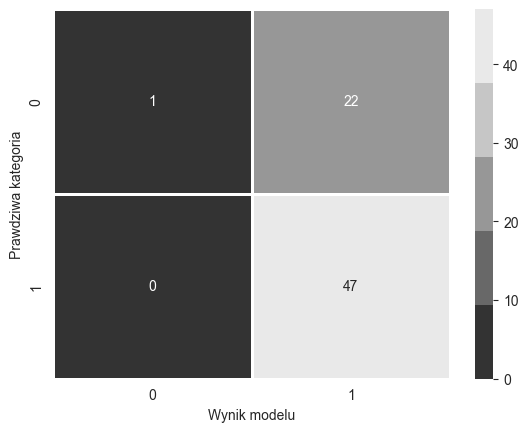
\includegraphics[width=\columnwidth]{thesis/assets/confusion_matrix_placeholder.png}
%         \caption{Sieć gęsta – Napięcia}
%         \label{fig:computer-time}
%     \end{subfigure}   
%     \hfill
%     \begin{subfigure}[b]{0.45\textwidth}
%         \centering
%         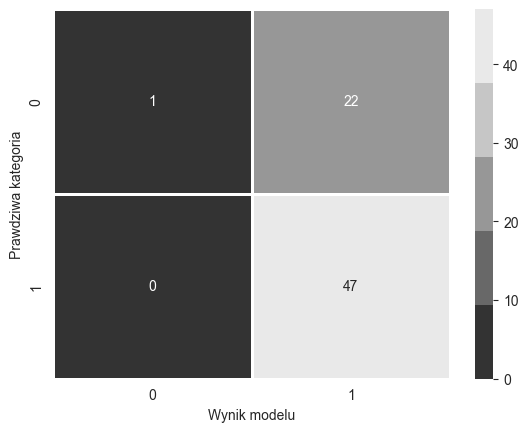
\includegraphics[width=\columnwidth]{thesis/assets/confusion_matrix_placeholder.png}
%         \caption{Sieć gęsta – Częstotliwości}
%         \label{fig:psychoactive-substances}
%     \end{subfigure}
%     \begin{subfigure}[b]{0.45\textwidth}
%         \centering
%         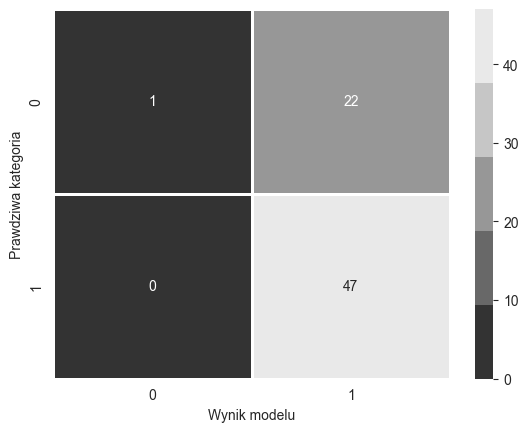
\includegraphics[width=\columnwidth]{thesis/assets/confusion_matrix_placeholder.png}
%         \caption{Sieć konwolucyjna – Napięcia}
%         \label{fig:computer-time}
%     \end{subfigure}   
%     \hfill
%     \begin{subfigure}[b]{0.45\textwidth}
%         \centering
%         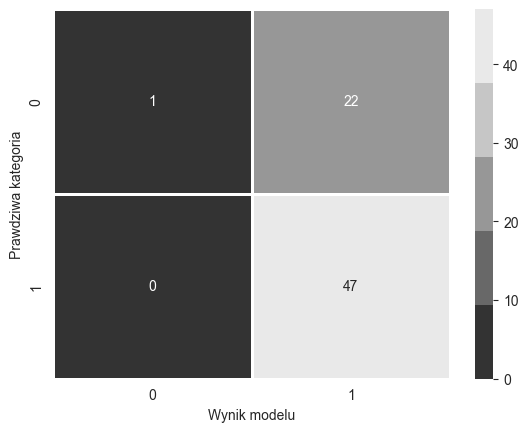
\includegraphics[width=\columnwidth]{thesis/assets/confusion_matrix_placeholder.png}
%         \caption{Sieć konwolucyjna – Częstotliwości}
%         \label{fig:psychoactive-substances}
%     \end{subfigure}
%     \begin{subfigure}[b]{0.45\textwidth}
%         \centering
%         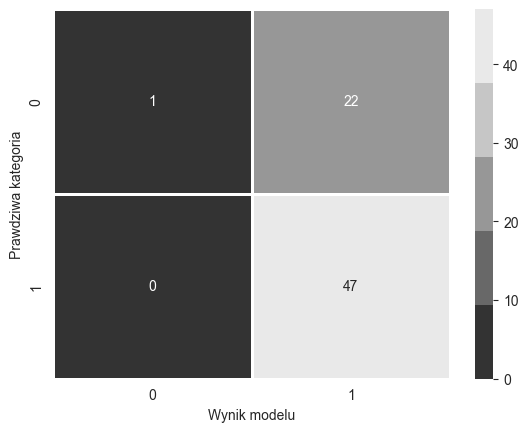
\includegraphics[width=\columnwidth]{thesis/assets/confusion_matrix_placeholder.png}
%         \caption{MLSTM – Częstotliwości}
%         \label{fig:computer-time}
%     \end{subfigure}   
%     \hfill
%     \begin{subfigure}[b]{0.45\textwidth}
%         \centering
%         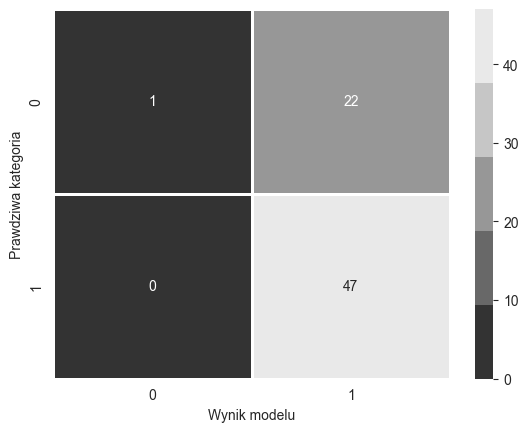
\includegraphics[width=\columnwidth]{thesis/assets/confusion_matrix_placeholder.png}
%         \caption{MLSTM – Napięcia}
%         \label{fig:psychoactive-substances}
%     \end{subfigure}
%     \caption{Macierze błędów}
%     \label{fig:confusion-matricies}
% \end{figure}

% \section{Analiza uprzedzeń algorytmicznych}\label{bias}
% % - wiek
% % - plec
% % - Perform statistical significance tests on the output of the network on a differing validation test


% W celu analizy ewentualnych uprzedzen algorytmicznych 

\section{Dyskusja}\label{dyskusja}
Pomimo statystycznie istotnej różnicy pomiędzy sygnałami odczytywanymi w czasie skupienia i spoczynku, zastosowane modele uczenia maszynowego nie wykazały zdolności do wykrycia tej zależności na oddzielonej populacji kontrolnej. Wyniki te, mimo zastosowania architektur \cite{} i metod trenowania modeli \cite{} o potwierdzonej skuteczności i zgodnych z najnowszymi osiągnięciami w dziedzinie uczenia maszynowego, sugerują niewystarczającą wielkość zbioru badawczego. Hipoteza niepoprawnego wykonania pomiarów odrzucona została ze względu na wykrywalną statystycznie różnice pomiędzy badanymi stanami. Niespodziewanie wysokie wariacje wprowadzone przez zbadane zmienne zakłócające wydają się wspierać niewystarczającą wielkość zbioru. Jednocześnie badania zaprezentowane w \cite{} przy zachowaniu podobnej ilości uczestników osiągają stanowczo lepsze rezultaty. Spowodowane mogło to być wykorzystaniem urządzeń pomiarowych przeznaczonych do użytku medycznego, a w związku z tym osiągnięcie wyższego efektywnego stosunku sygnału do szumu. W celu jednoznacznego zweryfikowania tezy badawczej wymagane jest zebranie większej ilości danych przez przeprowadzenie dodatkowej kampanii badawczej.

\printbibliography

\clearpage
\listoffigures
\clearpage
\listoftables
\clearpage
\lstlistoflisting
\clearpage

\appendix
\chapter{Formularze dla osób badanych}\label{formularz-dla-osoby-badanej}

\begin{figure}[h!]
    \centering
    \fbox{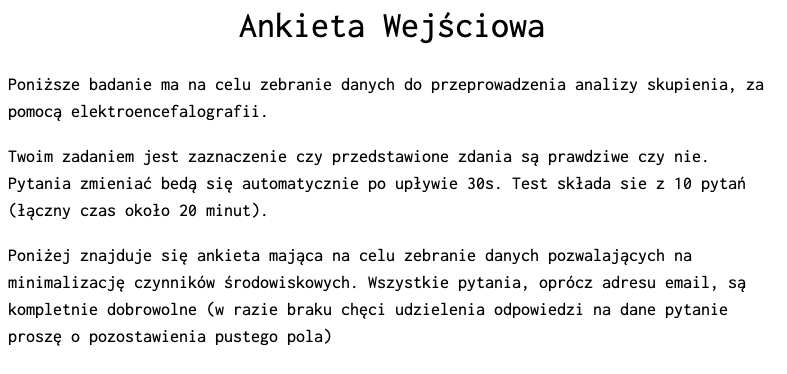
\includegraphics[width=\columnwidth]{thesis/assets/description_2.png}}
    \caption{Opis badania prezentowany ochotnikowi cz.1}
    \label{opis-badania}
\end{figure}

\begin{figure}[h!]
    \centering
    \fbox{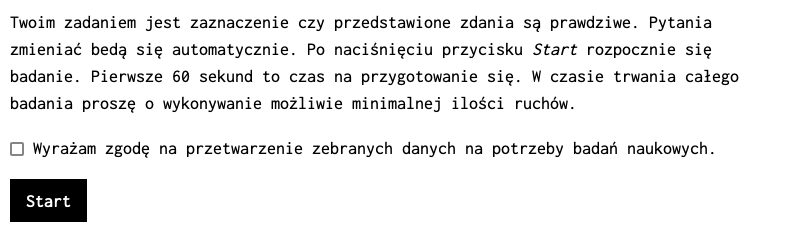
\includegraphics[width=\columnwidth]{thesis/assets/description_1.png}}
    \caption{Opis badania prezentowany ochotnikowi cz.2}
    \label{zgoda-na-przetwarzanie-danych}
\end{figure}


\begin{figure}[h!]
    \centering
    \fbox{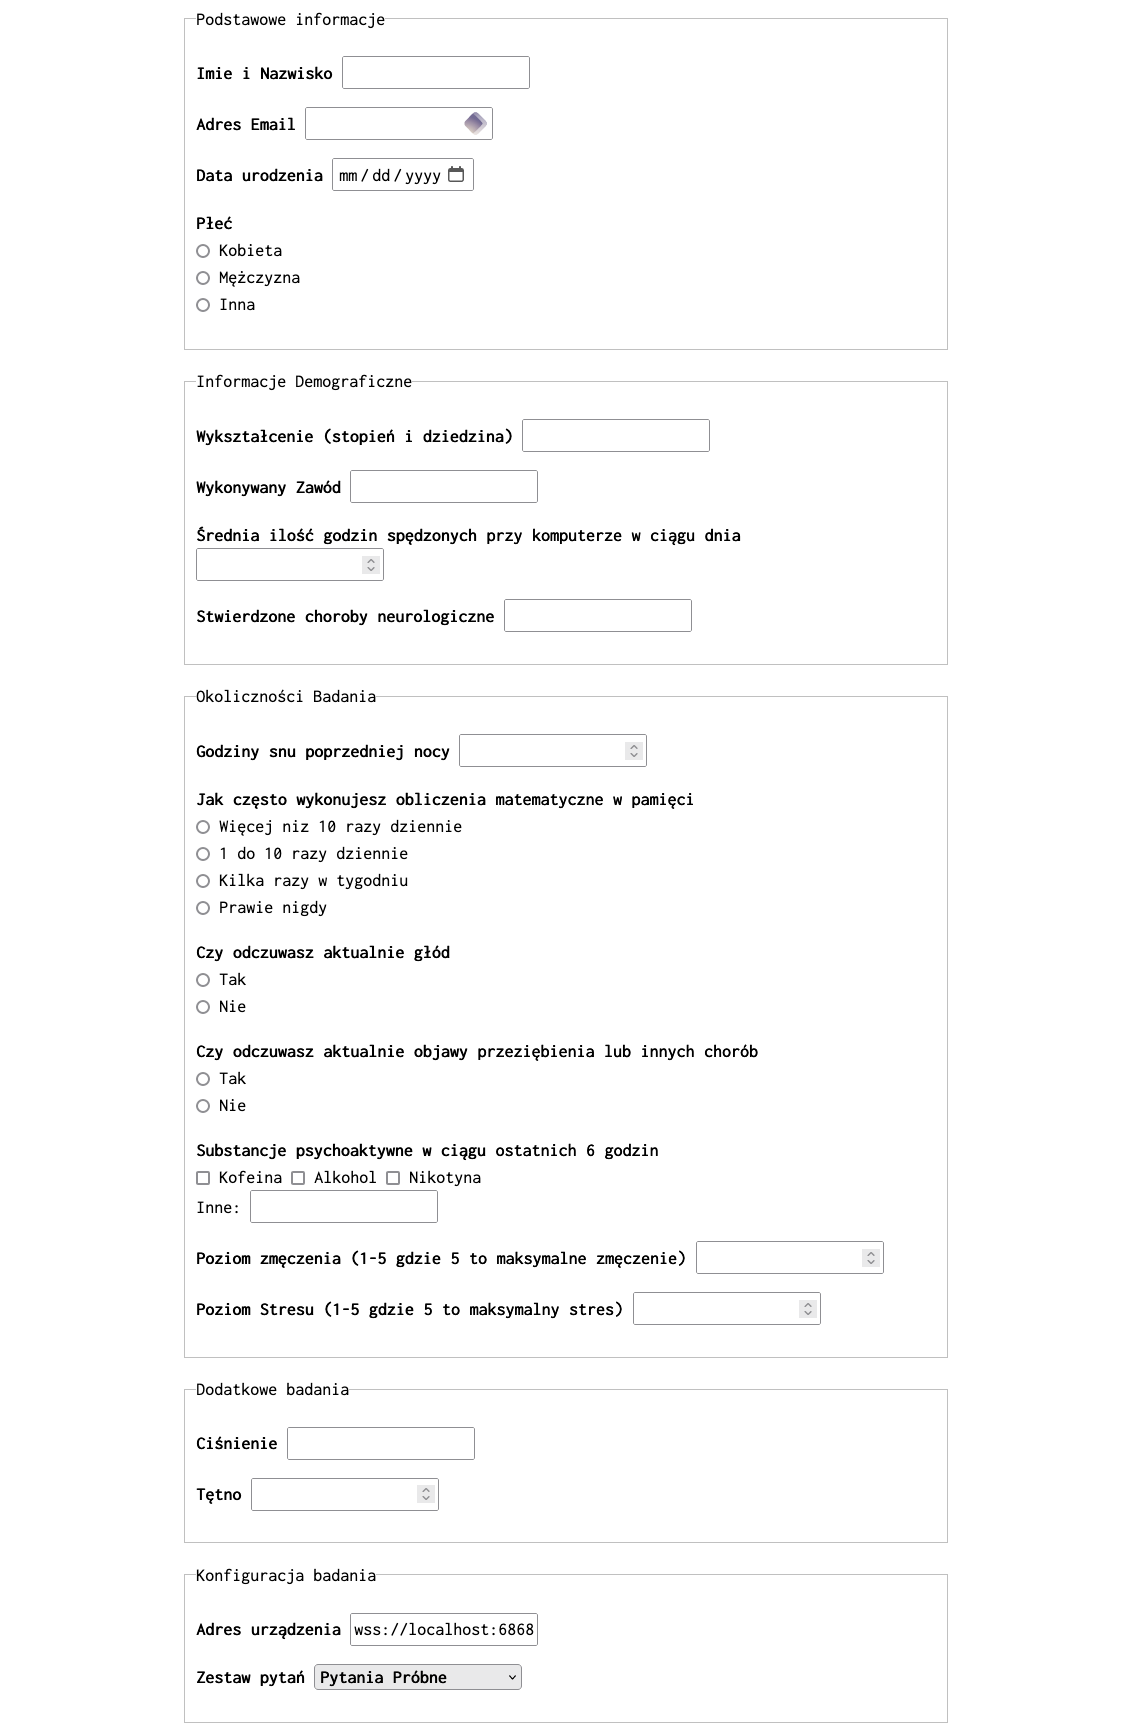
\includegraphics[width=\columnwidth]{thesis/assets/ankieta_wejsciowa.png}}
    \caption{Ankieta wstępna prezentowana przed rozpoczęciem badania}
    \label{pytania-ankiety-wejsciowej}
\end{figure}

\clearpage

% \begin{table}[h]
%     \centering
%     \begin{tabular}{|c|c|c|}
%         \hline
%         Pytanie \\
%         \hline
%         $(12*13)-11=145$ \\
%         $7*8*3=177$ \\
%         $\frac{121}{11}+39=50$ \\
%         $17+18+15+34=85$ \\
%         $8*6*5=240$ \\
%         $15*16*7=1680$ \\
%         $(17*17)+2=290$ \\
%         $173+(288*2)=750$ \\
%         $(89*3)+13=280$ \\
%         $7*7*7=343$ \\
%         \hline
%     \end{tabular}
%     \caption{Pytania zadawane podczas badania}
%     \label{pytania-badania}
% \end{table}

\begin{lstlisting}[caption={Plik konfiguracji wyświetlanych pytań},label={pytania-badania}]
[
    { "question": "Trwa kalibracja nie ruszaj się", "answerable": false },
    { "question": "$$(12*13)-11=145$$", "answerable": true },
    { "question": "$$7*8*3=177$$", "answerable": true },
    { "question": "$$\\frac{121}{11}+39=50$$", "answerable": true },
    { "question": "$$17+18+15+34=85$$", "answerable": true },
    { "question": "$$8*6*5=240$$", "answerable": true },
    { "question": "$$15*16*7=1680$$", "answerable": true },
    { "question": "$$(17*17)+2=290$$", "answerable": true },
    { "question": "$$173+(288*2)=750$$", "answerable": true },
    { "question": "$$(89*3)+13=280$$", "answerable": true },
    { "question": "$$7*7*7=343$$", "answerable": true },
    { "question": "Trwa kalibracja nie ruszaj się", "answerable": false }
]
\end{lstlisting}


\chapter{Instrukcja obsługi}\label{instrukcja}
\section{Wymagania systemowe}
\section{Instalacja}
\section{Obsługa}
\section{Konfiguracja}
\chapter{Dokumentacja API}\label{api}

\begin{boxA}
\textbf{\texttt{GET /api/cos}}

It is just a frame surrounded by a slightly thick line. A simple monochrome design might be fine, but when you want a gorgeous look, it's a bit unsatisfactory.
\end{boxA}

% - register questions endpoint
% - register answer
% - mark point
\end{document}